% -*- mode:flyspell; mode:latex -*-
\documentclass[12pt]{article}
\addtolength{\oddsidemargin} {-0.885in}
\addtolength{\textwidth}{1.75in}
\addtolength{\evensidemargin}{-0.8in}


\usepackage[latin1]{inputenc}
\usepackage[T1]{fontenc}
\usepackage[english]{babel}
\usepackage{graphicx}
\usepackage{float}
%% \usepackage{siunitx}

%% \usepackage{gensymb}


\usepackage{tikz}
\usepackage{[caption}
\usetikzlibrary{arrows}
\usetikzlibrary{decorations.markings}
\usetikzlibrary{decorations.pathmorphing}
% \usepackage[absolute,overlay]{textpos}
% \usepackage{onimage}

\usepackage{tabularx}
\usepackage{times}
\usepackage{graphics}

% \usepackage{subfigure}
% \usepackage{scalefnt}
%
% \renewcommand\thesubfigure{\arabic{subfigure}}

\usepackage{amsmath}
\usepackage{hyperref}
\usepackage{hhline}
\usepackage{subfig}
\usepackage{color}
\usepackage[all]{hypcap}

\usepackage[normalem]{ulem}  % for striking out
\usepackage{soul}
% \usepackage{fancyhdr}
% \pagestyle{fancy}
% \fancyhead[C]{}
% \fancyhead[L] {\it{Mu2e-doc-29670-v1.0} }
%%%%%%%%%%%%%%%%%%%%%%%%%%%%%%%%%%%%%%%%%%%%%%%%%%%%%%%%%%%%%%%%%%%%%%%%%%%%%%
% use natbib - biblatex not available on Mu2e interactive nodes
%%%%%%%%%%%%%%%%%%%%%%%%%%%%%%%%%%%%%%%%%%%%%%%%%%%%%%%%%%%%%%%%%%%%%%%%%%%%%%
\usepackage[square,sort,comma,numbers]{natbib}

% location of the .bib files: env var BIBINPUTS (~/library/bibliography)

% \usepackage[backend=biber, style=numeric-comp, sorting=ynt] {biblatex}
% \addbibresource{clfv.bib}

% \addbibresource{stntuple.bib}
% \addbibresource{mu2e_web.bib}
% \addbibresource{radiative_pion_capture.bib}

\graphicspath{{figures}}
%%%%%%%%%%%%%%%%%%%%%%%%%%%%%%%%%%%%%%%%%%%%%%%%%%%%%%%%%%%%%%%%%%%%%%%%%%%%%%
% for portability, make sure all commands are included locally,
%%%%%%%%%%%%%%%%%%%%%%%%%%%%%%%%%%%%%%%%%%%%%%%%%%%%%%%%%%%%%%%%%%%%%%%%%%%%%%
\definecolor{ForestGreen}{RGB}{20,109,20}
%%%%%%%%%%%%%%%%%%%%%%%%%%%%%%%%%%%%%%%%%%%%%%%%%%%%%%%%%%%%%%%%%%%%%%%%%%%%%%%
\newcommand {\abseta}    {\mbox{$\mid \eta \mid $}}
\newcommand {\Au}[1]     {\mbox{$\rm ^{#1}Au$}}          % isotopes of gold

\newcommand {\baftwo}    {\mbox{$BaF_2$}}
\newcommand {\blue}      {\color{blue}}

\newcommand {\deltaE}    {\mbox{$\delta{\rm-electron}$}}

\newcommand {\eemm}      {\mbox{$ee\mu\mu$}}
\newcommand {\emfr}      {\mbox{$\epsilon_{EM}$}}
\newcommand {\eminus}    {\mbox{$e^-$}}
\newcommand {\eplus}     {\mbox{$e^+$}}
\newcommand {\et}        {\mbox{$E_t$}}
\newcommand {\etcorr}    {\mbox{$E_T^{corr}$}}
\newcommand {\etaa}      {\mbox{$\eta$}}

\newcommand {\green}     {\color{ForestGreen}}
\newcommand {\gt}        {\mbox{$>$}}
\newcommand {\gea}       {\mbox{$>=$}}
\newcommand {\gevcsq}    {\mbox{$GeV\!/c^2$}}

\newcommand {\invfb}     {\mbox{$fb^{-1}$}}
\newcommand {\invfbrm}   {\mbox{$\rm fb^{-1}$}}
\newcommand {\invpb}     {\mbox{$pb^{-1}$}}
\newcommand {\invpbrm}   {\mbox{$\rm pb^{-1}$}}
\newcommand {\Ir}[1]     {\mbox{$\rm ^{#1}Ir$}}                 % isotopes of iridium

\newcommand {\jpsi}      {\mbox{$J/\psi$}}

\newcommand {\keVc}      {\mbox{$\rm keV\!/\!c$}}
\newcommand {\kmax}      {\mbox{$k_{\rm max}$}}

\newcommand {\lea}       {\mbox{$<=$}}
\newcommand {\lt}        {\mbox{$<$}}

\newcommand {\mcluster}  {\mbox{$M_{cluster}$}}
\newcommand {\met}       {\mbox{${\not\! E}_{T}$}}
\newcommand {\MeVc}      {\mbox{$\rm MeV\!/c$}}
\newcommand {\MeVcsq}    {\mbox{$\rm MeV\!/c^2$}}
\newcommand {\mmmm}      {\mbox{$\mu\mu\mu\mu$}}
\newcommand {\mt}        {\mbox{$E_{T}$ }}
\newcommand {\mtrkpi}    {\mbox{${M}_{trk+{\pi^0}'s}$ }}

% \newcommand {\mumemconv} {\mbox{$\mu^- A \rightarrow e^- A$}}
% \newcommand {\mumepconv} {\mbox{$\mu^- A \rightarrow e^+ A$}}

\newcommand \mumepconvRelay[1][A]  {\mbox{$\mu^- \textrm{\ArgI} \rightarrow e^+ \textrm{#1}$}}
\newcommand {\MuToEm}     {\mbox{$\mu^- \ra e^-$}}
\newcommand {\MuToEp}     {\mbox{$\mu^- \ra e^+$}}
\newcommand {\MuPToEp}    {\mbox{$\mu^+ \ra e^+$}}

\newcommand {\mumemconv}[1][A] {\mbox{$\mu^- \textrm{#1} \rightarrow e^- \textrm{#1}$}}
% Define a relay to have 2 default arguments instead of limit of 1
\newcommand {\mumepconv}[1][A] {%
  \def\ArgI{{#1}}%store the first argument
  \mumepconvRelay
}

\newcommand {\mzz}       {\mbox{$M_{ZZ}$}}

\newcommand {\pb}        {\mbox{\rm\,pb}}
\newcommand {\Pb}[1]     {\mbox{$\rm ^{#1}Pb$}}           % isotopes of lead: \Pb[208]

\newcommand {\pbar}      {\mbox{$\bar{p}$}}
\newcommand {\pizero}    {\mbox{$\pi^0$}}
\newcommand {\piplusenu} {\mbox{$\pi^+ \to e^+ \nu$}}
\newcommand {\pfake}     {\mbox{$P_{fake}$}}
\newcommand {\ppbar}     {\mbox{$p\bar{p}$}}
\newcommand {\ppbarw}    {\mbox{$p\bar{p} \rightarrow W$}}
\newcommand {\pt}        {\mbox{$P_t$ }}
\newcommand {\purple}    {\color{purple}}

\newcommand {\ra}        {\mbox{$\rightarrow$}}
\newcommand {\red}       {\color{red}}
\newcommand {\Rmue}      {\mbox{$R_{\mu e}$}}

\newcommand {\stat}          {\mbox{\rm (stat.)}}
\newcommand {\statsys}       {\mbox{\rm (stat.+syst.)}}
\newcommand {\syst}          {\mbox{\rm (syst.)}}

\newcommand {\tauenunu}  {\mbox{$\tau \ra e \nu \bar{\nu}$}}
\newcommand {\taumununu} {\mbox{$\tau \ra \mu \nu \bar{\nu}$}}
\newcommand {\tandip}    {\mbox{$\tan \lambda$}}
\newcommand {\ttau}      {\mbox{$\tau$}}
\newcommand {\Tau}       {\mbox{$\tau$}}

\newcommand {\violet}    {\color{violet}}
\newcommand {\vprop}     {\mbox{$v_{prop}$}}

\newcommand {\upar}      {\mbox{$u_{||}$}}
\newcommand {\uperp}     {\mbox{$u_{perp}$}}

\newcommand {\wenu}      {\mbox{$W\rightarrow e\nu$}}
\newcommand {\wlnu}      {\mbox{$W\rightarrow l\nu$}}
\newcommand {\wmunu}     {\mbox{$W\rightarrow \mu \nu$}}
\newcommand {\wpigamma}  {\mbox{$W^{\pm} \rightarrow \pi^{\pm} \gamma$}}
\newcommand {\wtaunu}    {\mbox{$W\rightarrow\tau\nu$}}

\newcommand {\zee}       {\mbox{$Z \rightarrow e^{+}e^{-}$}}
\newcommand {\zll }      {\mbox{$Z       \rightarrow l^{+}l^{-}$}}
\newcommand {\zmumu}     {\mbox{$Z \rightarrow \mu^{+}\mu^{-}$}}
\newcommand {\znunu}     {\mbox{$Z \rightarrow \nu\nu$}}
\newcommand {\zpsigamma} {\mbox{$    Z^{0} \rightarrow J/\psi \gamma$}}
\newcommand {\zpigamma}  {\mbox{$\rm Z^{0} \rightarrow \pi^{0} \gamma$}}
\newcommand {\ztautau}   {\mbox{$Z \rightarrow \tau\tau$}}
\newcommand {\zupsgamma}     {\mbox{$    Z^0 \rightarrow \Upsilon \gamma$}}
\newcommand {\zzx }          {\mbox{$X       \to ZZ$}}
\newcommand {\zzllll}        {\mbox{$ZZ \to \ell^+ \ell^- \ell^+ \ell^-$}}
\newcommand {\zzllnn}        {\mbox{$ZZ \to \ell^+ \ell^- \nu \nu$}}
\newcommand {\zzlljj}        {\mbox{$ZZ \to \ell^+ \ell^- j j$}}
%%%%%%%%%%%%%%%%%%%%%%%%%%%%%%%%%%%%%%%%%%%%%%%%%%%%%%%%%%%%%%%%%%%%%%%%%%%%%%
% editing commands
%%%%%%%%%%%%%%%%%%%%%%%%%%%%%%%%%%%%%%%%%%%%%%%%%%%%%%%%%%%%%%%%%%%%%%%%%%%%%%
\newcommand {\add}[1]    {{\red         {#1}}}
\newcommand {\strike}[1] {{\blue   \sout{#1}}}
\newcommand {\del}[1]    {{\blue   \sout{#1}}}
\newcommand {\dlt}[1]    {{\violet \sout{#1}}}   %alternate delete color
\newcommand {\hlite}[1]  {{\red      \ul{#1}}}   % needs xcolor, soul
%%%%%%%%%%%%%%%%%%%%%%%%%%%%%%%%%%%%%%%%%%%%%%%%%%%%%%%%%%%%%%%%%%%%%%%%%%%%%%%

% %%%%%%%%%%%%%%%%%%%%%%%%%%%%%%%%%%%%%%%%%%%%%%%%%%%%%%%%%%%%%%%%%%%%%%%%%%%%%%
% for editors
% %%%%%%%%%%%%%%%%%%%%%%%%%%%%%%%%%%%%%%%%%%%%%%%%%%%%%%%%%%%%%%%%%%%%%%%%%%%%%%
\newcommand {\pasha}[1]     {{\green  #1}}
\newcommand {\simon}[1]     {{\blue   #1}}
%%%%%%%%%%%%%%%%%%%%%%%%%%%%%%%%%%%%%%%%%%%%%%%%%%%%%%%%%%%%%%%%%%%%%%%%%%%%%%
\begin{document}

\begin{titlepage}
  \begin{flushright}
    \bf {MU2E/PHYSICS/50071} \\
    version 1.02
    \today
 \end{flushright}

  \vspace{1cm}

  \begin{center}
    {\Large \bf MIDAS+ARTDAQ-based data acquisition system for Mu2e
      \vspace{0.3in}
    }

    \vspace{1cm}
    S.Corrodi(ANL), A.Keshavarzi (Manchester) P.Murat(FNAL), ...

    % \footnote{\texttt{Fermilab; e-mail: murat@fnal.gov}}
    \vspace{0.3cm}

    \vspace{0.8cm}
  \end{center}

  \begin{abstract}
    \vspace{0.2in}

    Over the last several months, several Mu2e subdetector groups have extensively
    prototyped a solution for the Mu2e data acquisition system based on MIDAS+ARTDAQ.
%
    The functionality of the prototyped system in many aspects, already exceeds that
    of the OTSDAQ-based DAQ used in the GR3, and the prototyped system is much simpler
    from the user as well as from the developer prospective.
    
    \vspace{0.2in}
    We propose to exercise this solution in the upcoming GR4.
    
  \end{abstract}

\end{titlepage}
% \frontmatter
% \chapter*{Abstract}
%
% \addcontentsline{toc}{chapter}{Abstract}
%
% \mainmatter
%
{\tableofcontents}

%%%%%%%%%%%%%%%%%%%%%%%%%%%%%%%%%%%%%%%%%%%%%%%%%%%%%%%%%%%%%%%%%%%%%%%%%%%%%%%
%\chapter{Calibration}
%%%%%%%%%%%%%%%%%%%%%%%%%%%%%%%%%%%%%%%%%%%%%%%%%%%%%%%%%%%%%%%%%%%%%%%%%%%%%%%
% \input{input_data}

%%%%%%%%%%%%%%%%%%%%%%%%%%%%%%%%%%%%%%%%%%%%%%%%%%%%%%%%%%%%%%%%%%%%%%%%%%%%%%%
\newpage
\section {Revision History and TODO items}

\begin{itemize}
\item
  v1.01: version for internal review
\end{itemize}

% {\red
% TODO items:
% 
% \begin{itemize}
% \item
% \end{itemize}
% }
%%%%%%%%%%%%%%%%%%%%%%%%%%%%%%%%%%%%%%%%%%%%%%%%%%%%%%%%%%%%%%%%%%%%%%%%%%%%%%
\newpage
\section {Executive Summary}

Development of the Mu2e DAQ has been lagging behind for quite significant time.
Despite some recent progress, after years of trying no Mu2e collaborator
can operate the DAQ system in their own. With a few months left before the start of the
cosmic run, the system has missing pieces which are yet to be designed.
%
The core of the DAQ system, OTSDAQ, has not been used before by any running experiment.
In is complicated and undocumented. The interfaces between different parts are not
specified, and its complexity and lack of modularity create a very high entry
threshold for the Mu2e collaborators.
%
Most of the DAQ development is happening outside the collaboration which has very
limited input into the development process.
%
During the data taking, the collaboration will have to operate the DAQ system
and it will have to be functional 24x7. In our view, the cost of operating 
and supporting the present DAQ system, expressed in terms of the lost beam time,
will be too high.

% 
We have therefore developed and prototyped a DAQ system based on the combination of two
packages, ARTDAQ \cite{2017_ARTDAQ_Biery} and MIDAS \cite{2025_MIDAS_WIKI}.
%
ARTDAQ is a distributed trigger farm software developed at Fermilab and previously
used by several Fermilab neutrino experiments. 
%
MIDAS is a full DAQ suite which has been used for about 30 years by many HEP experiments
at PSI, TRIUMF, CERN, KEK. It should be noted that MIDAS has also been used
by the g-2 experiment at Fermilab.
%
Out of the currently running experiments, MIDAS is currently used by MEG-II which,
as Mu2e,  searches for CLFV. Another CLFV experiment, Mu3e, which DAQ hardware architecture
is rather close to that of Mu2e, will also be using a MIDAS-based DAQ system.
In a way, MIDAS became a de-facto DAQ standard for small and medium scale HEP
experiments.

Any DAQ system at its early stages has many issues which can only be uncovered and fixed
by operating it. MIDAS has been debugged and tuned by tens of experiments
and by decades of the running time. Although the initial design of MIDAS goes 30 years back,
its architecture is advanced, and the software infrastructure is constantly updated
to use modern technologies.

Based on our technical assessment, the proposed system which combines
the distributed data processing by ARTDAQ with the integrated MIDAS-based
run control and monitoring, provides the best technical solution for the Mu2e DAQ.
In many aspects, its functionality already exceeds the functionality of the OTSDAQ.
%
Adding to that, many Mu2e collaborators already have operational experience with
the MIDAS-based DAQ. New collaboration members, coming to Mu2e from other muon 
experiments will likely know MIDAS and would be able to operate the system and
contribute to its future development.
It should be noted, that students have already made important contribution
to the current development.

The following sections describe the architecture of the proposed system,
its interfaces, and the status of the implementation.

\section{System architecture}

The proposed system consists of two big software components :
\begin{itemize}
\item
  ARTDAQ : handles the trigger farm and the data processing
\item
  MIDAS : handles the run configuration, run control, messaging,
  standardizes interfaces between various parts of the online system,
  and provides web-based interface for the shifters,
\end{itemize}

The DAQ architecture is schematically presented in Figure ~\ref{figure:system_architecture}
\begin{figure}[H]
  \begin{tikzpicture}
    \node[anchor=south west,inner sep=0] at (0,0.) {
      % \node[shift={(0 cm,0.cm)},inner sep=0,rotate={90}] at (0,0) {}
      \makebox[\textwidth][c] {
        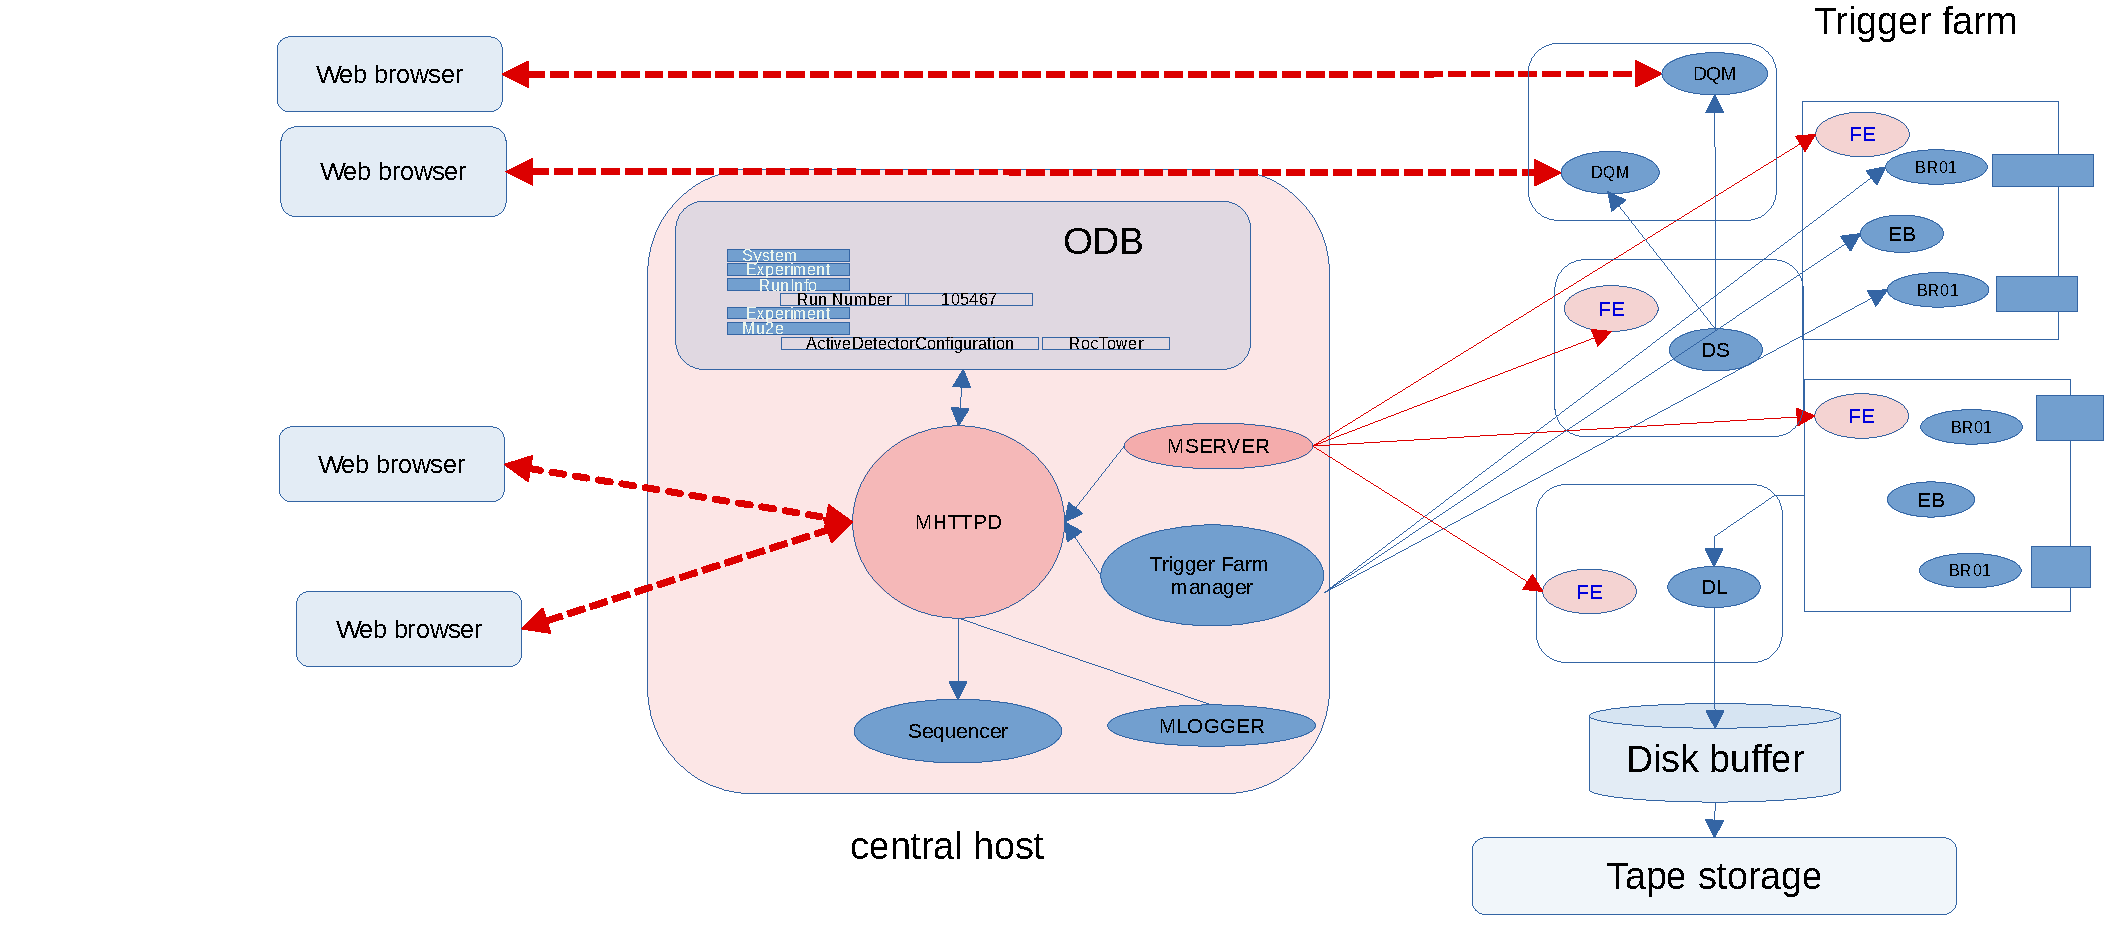
\includegraphics[width=1.1\textwidth]{pdf/system_architecture}
      }
    };
    % \node [text width=8cm, scale=1.0] at (14.5,0.5) {$\mu_B$, expected background mean};
    % \node [text width=8cm, scale=1.0, rotate={90}] at (1.5,7.5) { $S_{D}$, ``discovery'' signal strength  };
  \end{tikzpicture}
  \caption{
    \label{figure:system_architecture}
    Architecture of the MIDAS-based DAQ system
  }
\end{figure}

%%%%%%%%%%%%%%%%%%%%%%%%%%%%%%%%%%%%%%%%%%%%%%%%%%%%%%%%%%%%%%%%%%%%%%%%%%%%%%
\subsection{MIDAS}

COre parts of MIDAS are :

\begin{itemize}
\item 
  mhttpd, a web server with restricted functionality
  mhttpd connects its clients to ODB. 
  The mhttpd doesn't execute any applications. Instead, it only updates the ODB.
\item
  Clients: frontends, communicating with the hardware and other
  parts of the system. Different types of frontends. Mu2e only needs slow monitoring.
\item
  Online DataBase (ODB) - a shared memory segment, which stores all configuration data of the system. Despite its name, ODB is not a database. Instead, it stores only current configuration
  of the system, As the new run starts, a run number-stamped configuration is exported and stored.
  Logical organization of ODB maps onto a json structure and is well suited for describing
  complex configurations with multiple levels of hierarchy
\end{itemize}

MIDAS ODB has several interfaces:
\begin{itemize}
\item 
  web-based interface - via the mhttpd ODB page
\item
  command line interface (odbedit)
\item
  C++ interface allowing C++ clients to interact with ODB
\item
  python interface
\end{itemize}

In all cases, clients connect to MHTTPD and MHTTPD acts as
the only agent directly interacting with the ODB.

%%%%%%%%%%%%%%%%%%%%%%%%%%%%%%%%%%%%%%%%%%%%%%%%%%%%%%%%%%%%%%%%%%%%%%%%%%%%%%
\subsection{Frontends}

MIDAS supports frontends of different types, which include the data readout and monitoring
frontends.

MIDAS event building functionality is not used , done by ARTDAQ.

The architecture of the Mu2e DAQ requires only monitoring and slow control frontends.


%%%%%%%%%%%%%%%%%%%%%%%%%%%%%%%%%%%%%%%%%%%%%%%%%%%%%%%%%%%%%%%%%%%%%%%%%%%%%%
\subsection{Interface to ARTDAQ}
All high bandwidth traffic goes through ARTDAQ.

ARTDAQ processes are controlled by the Trigger Farm Manager (TFM) frontend,
tfm\_launch\_fe.py.

\begin{itemize}
\item 
  TFM reads its initial settings from the "/Mu2e/ActiveRunConfiguration/DAQ/Tfm"
  ODB configuration path.
\item
  FCL files of ARTDAQ processes are stored in \$MU2E\_DAQ\_DIR/config/\$run\_configuration
  subdirectory assumed to be the same (network mounted) on all DAQ nodes.
  The FCL files could be regenerated manually based on the run configuration and the trigger table.
\item
  Archival mechanism: the FCL files used for a given run are stored
  in \$DAQ\_OUTPUT\_TOP/run\_records/\$run\_number area of the node where the TFM frontend is running.
\item
  the log files of ARTDAQ processes running on a given node are stored in \$DAQ\_OUTPUT\_TOP/logs
  directory of that node
\end{itemize}

%%%%%%%%%%%%%%%%%%%%%%%%%%%%%%%%%%%%%%%%%%%%%%%%%%%%%%%%%%%%%%%%%%%%%%%%%%%%%%
\subsubsection{Naming conventions for ARTDAQ components}

It is assumed that :
\begin{itemize}
\item 
  artdaq boardreaders described in the configuration have names "br01", "br02", etc
\item 
  artdaq event builders have names "eb01", "eb02", etc
\item 
  artdaq data loggers have names "dl01", "dl02", etc
\item 
  artdaq dispatchers have names "ds01", "ds02", etc
\end{itemize}

This convention allows to use component names, as they are, in the monitoring system.

%%%%%%%%%%%%%%%%%%%%%%%%%%%%%%%%%%%%%%%%%%%%%%%%%%%%%%%%%%%%%%%%%%%%%%%%%%%%%%
\subsubsection{Port assignment for ARTDAQ XML-RPC communication}
\begin{itemize}
\item
  base\_port: 10000+1000*partition\_number
\item 
  TFM : base\_port
\item 
  MIDAS node monitoring frontend: base\_port+11;
\item 
  artdaq boardreaders: base\_port+101 and base\_port+102
\item 
  artdaq event builders : base\_port + 201 - base\_port+300;
\item 
  artdaq data loggers  : base\_port + 301 - base\_port+400;
\item 
  artdaq dispatchers : base\_port + 401 - base\_port+500
\end{itemize}


%%%%%%%%%%%%%%%%%%%%%%%%%%%%%%%%%%%%%%%%%%%%%%%%%%%%%%%%%%%%%%%%%%%%%%%%%%%
\subsubsection{Communication with ARTRAQ}

\begin{itemize}
\item
  native artdaq communication is internal to the ARTDAQ
\item
  ARTDAQ processes report their metrics in XML-RPC format,
  and it is assumed that parsing of the metrics, visualizing
  it and generating alarms is the job of the 3-rd party application,
  i.e. {\bf grafana}.
\item
  TFM queries the ARTDAQ process metrics over XML-RPC and records
  them in ODB. That obsoletes the need in the 3rd party applications.
\item
  Mu2e -specific applications, i.e. the boardreaders and the filter modules 
  communicate to the MIDAS server directly via messaging and report 
  their status. Therefore simple alarms like single ROC timeouts etc
  could be generated as they are detected. 
  This avoids a need in an additional software to recognize an alarming
  situation and trigger the corresponding notification mechanism.
\end{itemize}


%%%%%%%%%%%%%%%%%%%%%%%%%%%%%%%%%%%%%%%%%%%%%%%%%%%%%%%%%%%%%%%%%%%%%%%%%%%%%%
\subsection{Interface to the online run conditions database} 

\begin{itemize}
\item
  the interface is provided by the MIDAS Sequencer and 
  \href{https://github.com/pavel1murat/frontends/blob/main/conf/mu2e_config_fe.py}
  {\blue the global configuration frontend}.
\item
  before the TFM starts, the configuration frontend requests a new run 
  number from the run configuration DB.
\item
  at begin run, the TFM frontend passes the run number to ARTDAQ processes.
\item
  the global configuration frontend registers the start and the stop of each
  run transition in the run configuration database.
\end{itemize}


%%%%%%%%%%%%%%%%%%%%%%%%%%%%%%%%%%%%%%%%%%%%%%%%%%%%%%%%%%%%%%%%%%%%%%%%%%%%%% 
\subsection{Slow monitoring}

MIDAS history system provides the framework for slow monitoring.
The historical data could be stored in  MIDAS internal format or in a database.
The list of supported databases includes ODBC, SQLITE, MYSQL and PGSQL.

This functionality is similar to that of grafana, however integrated with the
rest of the system

\begin{itemize}
\item
  one monitoring frontend per node 
  \begin{itemize}
  \item
    controls and configures DTC's and ROCs on this node
  \item
    controls the CFO if the CFO is running on this node
  \item
    monitors DTCs and ROCs, collecting history and non-history information
  \item
    monitors artdaq processes d separate collection of the monitoring information and its visualization
  \end{itemize}
\end{itemize}

Figure ~\ref{figure:slow_controls_node_page} gives an example of one of the slow controls pages

\begin{figure}[H]
  \begin{tikzpicture}
    \node[anchor=south west,inner sep=0] at (0,0.) {
      % \node[shift={(0 cm,0.cm)},inner sep=0,rotate={90}] at (0,0) {}
      \makebox[\textwidth][c] {
        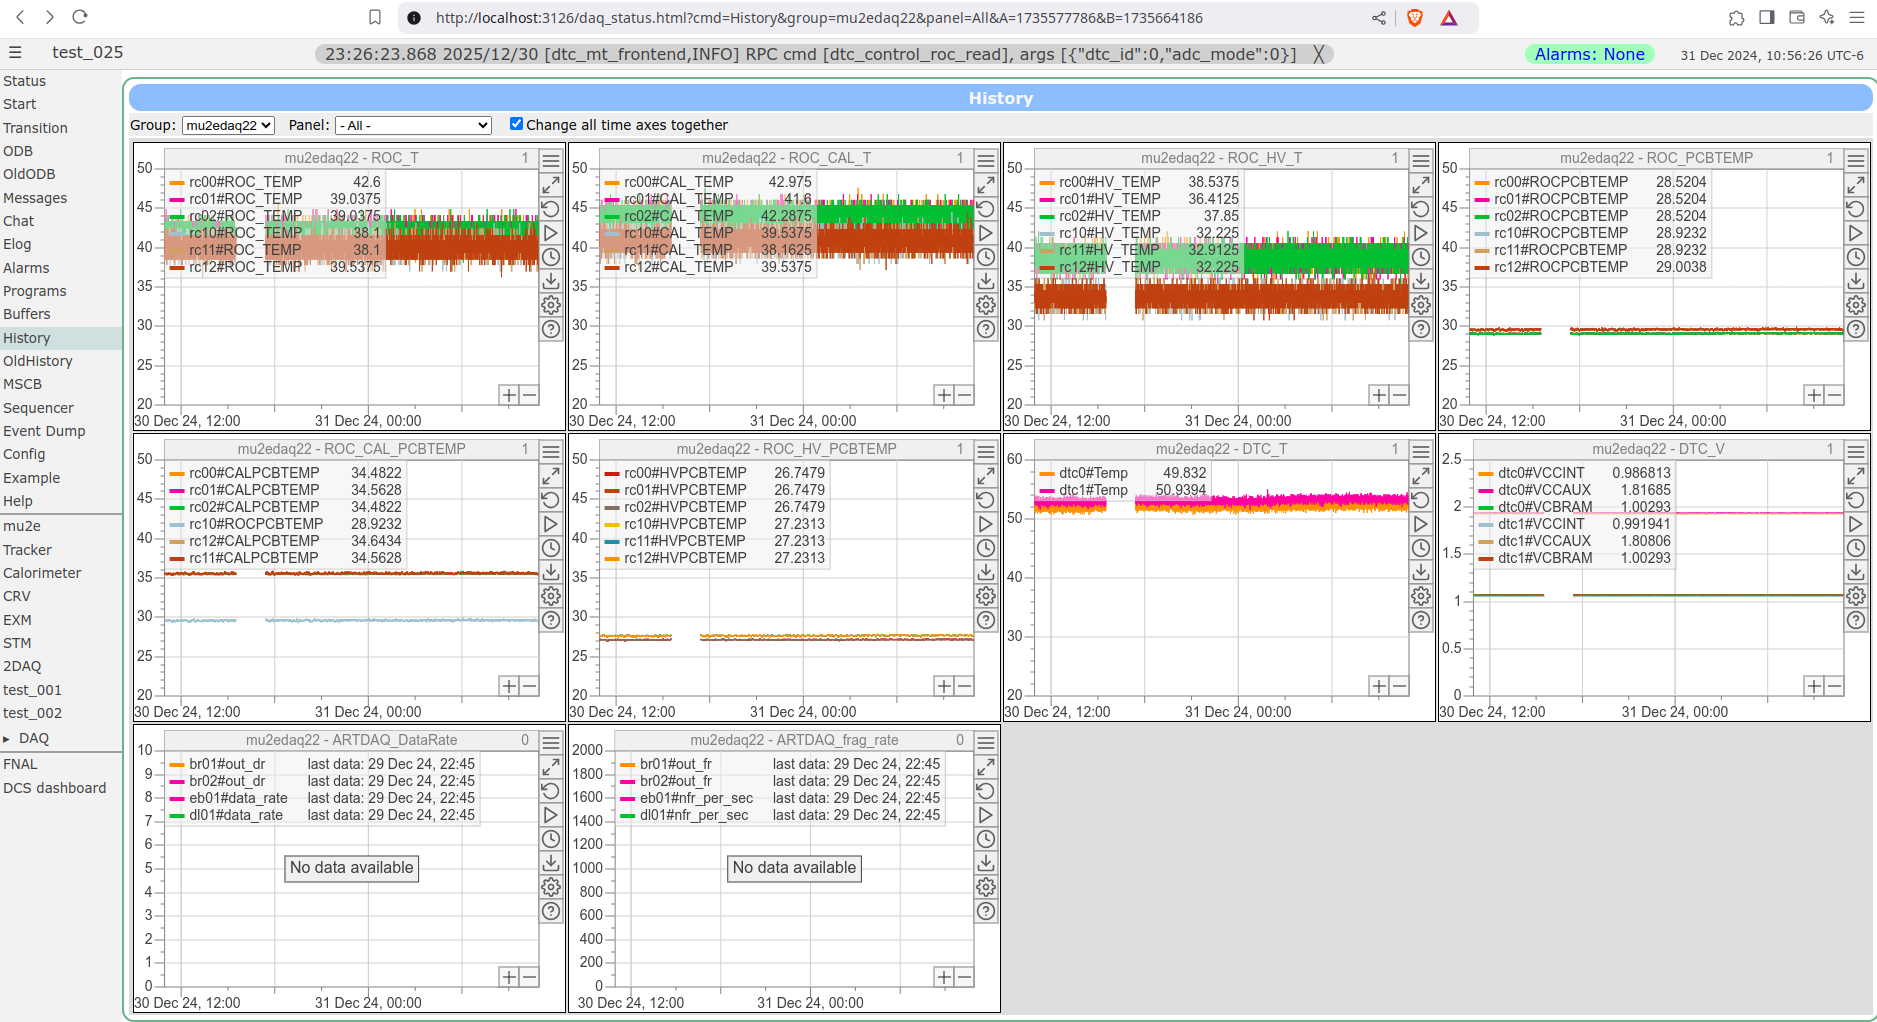
\includegraphics[width=0.95\textwidth]{png/slow_controls_node_page}
      }
    };
    % \node [text width=8cm, scale=1.0] at (14.5,0.5) {$\mu_B$, expected background mean};
    % \node [text width=8cm, scale=1.0, rotate={90}] at (1.5,7.5) { $S_{D}$, ``discovery'' signal strength  };
  \end{tikzpicture}
  \caption{
    \label{figure:slow_controls_node_page}
    A prototype of the DAQ node slow control page. Monitored are the DTC and ROC temperatures and voltages
    and rates of the ARTDAQ processes
  }
\end{figure}


%%%%%%%%%%%%%%%%%%%%%%%%%%%%%%%%%%%%%%%%%%%%%%%%%%%%%%%%%%%%%%%%%%%%%%%%%%%%%%
\subsection{Alarm system}

MIDAS has a built-in alarm system which could be used to inform shifters
about various categories of failures.

That is not a replacement for critical alarms coming from different inputs.
CRYO ? Accelerator ? -{\red talk to Andy Hocker.}


%%%%%%%%%%%%%%%%%%%%%%%%%%%%%%%%%%%%%%%%%%%%%%%%%%%%%%%%%%%%%%%%%%%%%%%%%%%%%% 
\subsection{Javascript web interface}

\begin{itemize}
\item 
  MIDAS web interface is a combination of HTML5+Javascript, based on the
  asynchronous approach to the web pages update (Ajax).
\item 
  MIDAS provides Javascript API to ODB, which facilitates development of
  functional experiment-specific {\bf custom} web pages.
  The interface is documented at \\
  \href{https://daq00.triumf.ca/MidasWiki/index.php/Custom\_Page}
  {\blue https://daq00.triumf.ca/MidasWiki/index.php/Custom\_Page}
\end{itemize}


%%%%%%%%%%%%%%%%%%%%%%%%%%%%%%%%%%%%%%%%%%%%%%%%%%%%%%%%%%%%%%%%%%%%%%%%%%%%%%
\subsection{Interfaces to ECL, ELOG, Slack}

MIDAS has interfaces to internal and external ELOGs and Slack.
\begin{itemize}
\item
  interface to the external ELOG has been implemented and tested
\item
  interface to Slack has been tested and used by at least two experiments - MEG and g-2
\item
  interface to ECL - to be implemented
\end{itemize}


%%%%%%%%%%%%%%%%%%%%%%%%%%%%%%%%%%%%%%%%%%%%%%%%%%%%%%%%%%%%%%%%%%%%%%%%%%%%%%
\subsection{Interface to EPICS}

Although MIDAS has its own history system , it also has an interface to EPICS,
implemented as a slow control frontend

%%% Local Variables:
%%% mode: latex
%%% TeX-master: t
%%% End:


%%%%%%%%%%%%%%%%%%%%%%%%%%%%%%%%%%%%%%%%%%%%%%%%%%%%%%%%%%%%%%%%%%%%%%%%%%%%%%
\subsection{DQM}

DQM processes use ROOT-based histogramming. As any ROOT executable is a web server,
the DAQM jobs publish their histograms on the web, and their clients (users)
simply connect to them over the http protocol.

%%%%%%%%%%%%%%%%%%%%%%%%%%%%%%%%%%%%%%%%%%%%%%%%%%%%%%%%%%%%%%%%%%%%%%%%%%%%%% 
\subsection{Interprocess communication} 

The system supports three mechanisms
\begin{itemize}
\item
  via ODB : some clients write into ODB, others read
\item
  separate collection of the monitoring information and its visualization
\item
  MIDAS messaging: jsonrpc.
  \begin{itemize}
  \item
    Each client can have a jsonrpc server and receive messages
    from any other client.
  \item
    clients can broadcast messages to the system (info and alarm)
    and communicate to each other
  \item
    each frontend, C++ or Python, has a built-in jsonrpc communication
    functionality built-in.
  \end{itemize}
\item
  communication between ARTDAQ processes is based on an older technology,
  XML-RPC. The TFM frontend supports the XML-RPC-based ARTDAQ communication
  protocol.
\end{itemize}

%%%%%%%%%%%%%%%%%%%%%%%%%%%%%%%%%%%%%%%%%%%%%%%%%%%%%%%%%%%%%%%%%%%%%%%%%%%%%%
\section{System configuration}

The proposed DAQ system supports multiple run configurations,
as shown in Figure~\ref{figure:run_configurations}.

\begin{figure}[H]
  \begin{tikzpicture}
    \node[anchor=south west,inner sep=0] at (0,0.) {
      % \node[shift={(0 cm,0.cm)},inner sep=0,rotate={90}] at (0,0) {}
      \makebox[\textwidth][c] {
        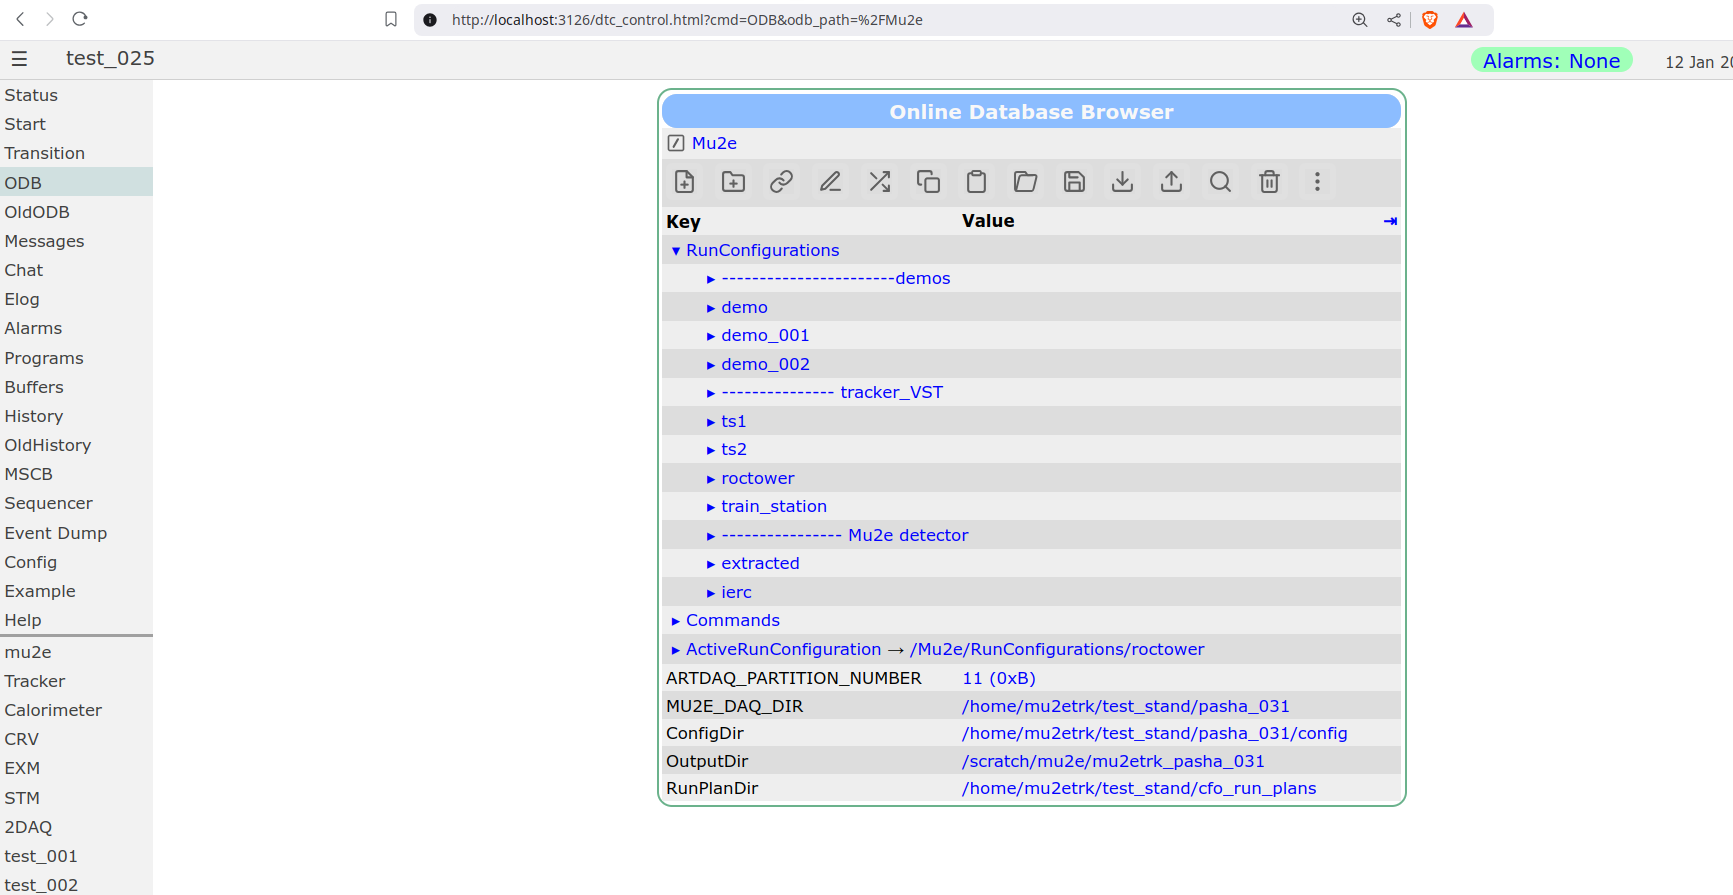
\includegraphics[width=0.95\textwidth]{png/run_configurations}
      }
    };
    % \node [text width=8cm, scale=1.0] at (14.5,0.5) {$\mu_B$, expected background mean};
    % \node [text width=8cm, scale=1.0, rotate={90}] at (1.5,7.5) { $S_{D}$, ``discovery'' signal strength  };
  \end{tikzpicture}
  \caption{
    \label{figure:run_configurations}
    Top-level run configurations
  }
\end{figure}

\begin{itemize}
\item 
  Run configurations are stored in the "/Mu2e/RunConfigurations" ODB subtree
\item
  each run configuration is an independent subtree, so any modification
  of a given run configuration doesn't affect other run configurations
\item
  a run configuration template can be saved as a .json structure and loaded from
  an external .json file, for example
\begin{verbatim}
mu2etrk@mu2edaq22:~/test_stand/pasha_031>odbedit
[local:test_025:S]/>cd Mu2e/Run
[local:test_025:S]/>cd Mu2e/RunConfigurations/demo
[local:test_025:S]demo>save demo.json
[local:test_025:S]demo>exit
\end{verbatim}
\item
  ODB links are allowed, but have to point within the configuration
\item
  configuration templates are archived on github. 
\end{itemize}

%%%%%%%%%%%%%%%%%%%%%%%%%%%%%%%%%%%%%%%%%%%%%%%%%%%%%%%%%%%%%%%%%%%%%%%%%%%%%%
\subsection{Structure of  the run configuration}
\begin{itemize}
\item 
  a run configuration has a name, a status, a list of elements - subsytem configurations,
  \new{and some global parameters,} as shown in Figure~\ref{figure:configuration_top}
\item
  each subsystem has a separate configuration subtree
\item
  \new{subsystem configuration templates are archived} in the 
  \href{https://github.com/pavel1murat/frontends/tree/main/odb/Mu2e/Subdetectors}
  {\blue frontends/odb/Mu2e/Subdetectors} subdirectory
\item
  Shown in  Figure~\ref{figure:run_configurations} ODB element "/Mu2e/ActiveRunConfiguration" is an ODB link
  pointing to the currently active configuration ("roctower").
\end{itemize}

\begin{figure}[H]
  \begin{tikzpicture}
    \node[anchor=south west,inner sep=0] at (0,0.) {
      % \node[shift={(0 cm,0.cm)},inner sep=0,rotate={90}] at (0,0) {}
      \makebox[\textwidth][c] {
        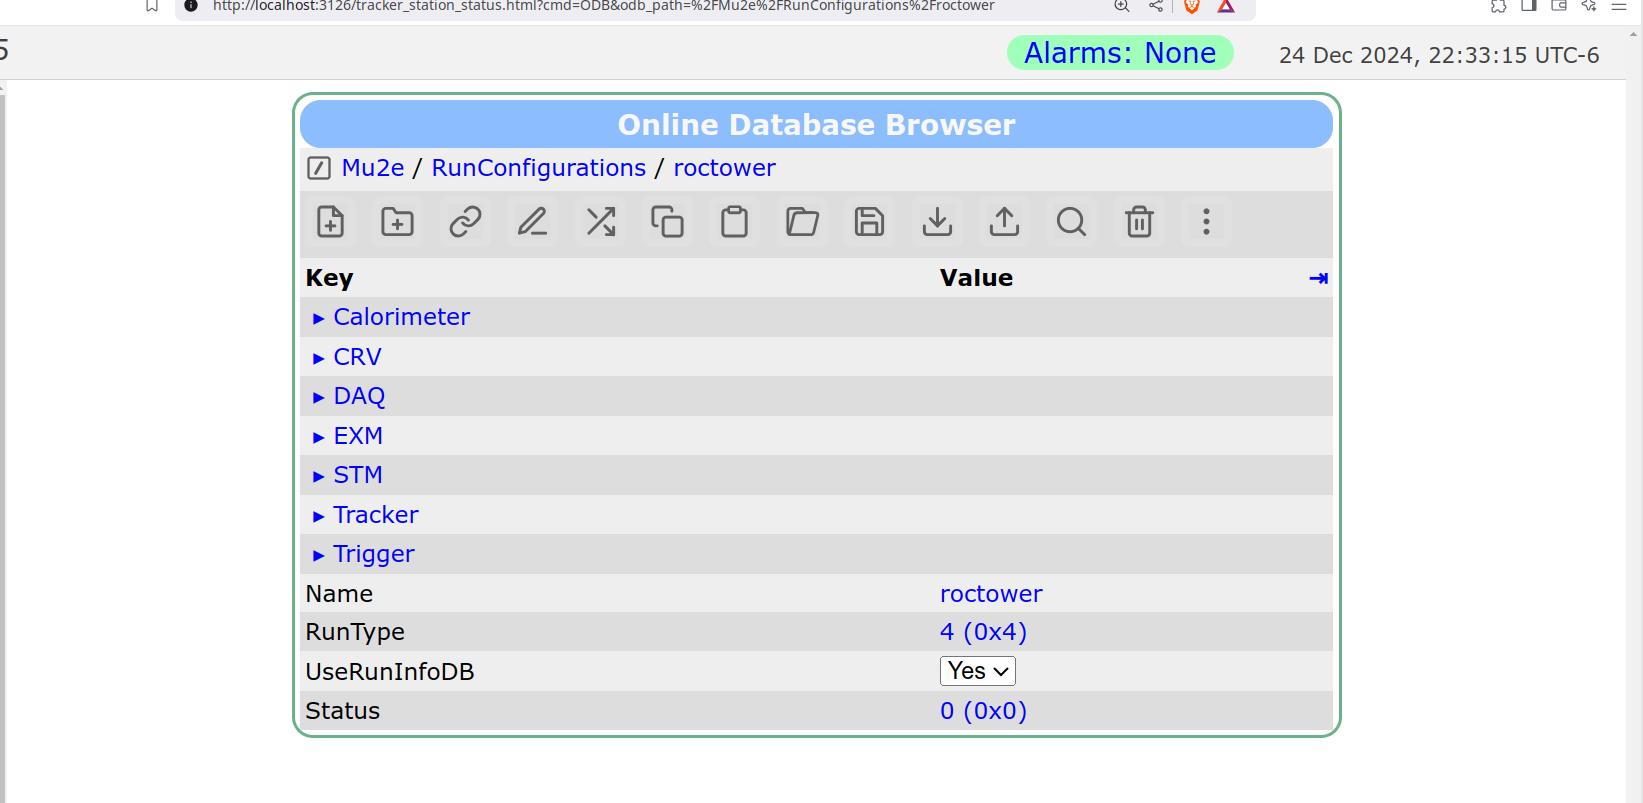
\includegraphics[width=0.95\textwidth]{png/configuration_top}
      }
    };
    % \node [text width=8cm, scale=1.0] at (14.5,0.5) {$\mu_B$, expected background mean};
    % \node [text width=8cm, scale=1.0, rotate={90}] at (1.5,7.5) { $S_{D}$, ``discovery'' signal strength  };
  \end{tikzpicture}
  \caption{
    \label{figure:configuration_top}
    Top view of the configuration called 'roctower' - a 6-ROC tracker test stand in IERC
  }
\end{figure}

%%%%%%%%%%%%%%%%%%%%%%%%%%%%%%%%%%%%%%%%%%%%%%%%%%%%%%%%%%%%%%%%%%%%%%%%%%%%%% 
\subsection{Subsystem configuration}

Each Mu2e subsystem, subdetectors and the DAQ, is represented by its
configuration [sub]tree in the detector configuration.
The configuration trees are subsystem-specific, consist of different elements,
and have different levels of hierarchy.
However, each configuration element has two mandatory parameters, {\bf Enabled}
and {\bf Status}, used for monitoring and error reporting.
Their meaning is as follows 

\begin{itemize}
\item
  {\bf Enabled} = 0: the element (sub-tree) is considered present, but not used.
\item
  {\bf Enabled} = 1: the element is included into the configuration and expected
  to be used
  \begin{itemize}
  \item
    status = 0 : the subsystem is OK
  \item
    status < 0 : the subsystem has a problem and an action is required
    The value of the status variable is the error code
  \item
    status > 0 : the subsystem has a warning-level problem, no immediate action
    is required
  \end{itemize}
\end{itemize}

The following sections describe configurations of the individual subsystems

%%% Local Variables:
%%% mode: latex
%%% TeX-master: t
%%% End:


%%%%%%%%%%%%%%%%%%%%%%%%%%%%%%%%%%%%%%%%%%%%%%%%%%%%%%%%%%%%%%%%%%%%%%%%%%%%%% .

\subsection{Tracker} 

A top view of the tracker configuration is shown in Figure~\ref{figure:tracker_config}.

\begin{figure}[H]
  \begin{tikzpicture}
    \node[anchor=south west,inner sep=0] at (0,0.) {
      % \node[shift={(0 cm,0.cm)},inner sep=0,rotate={90}] at (0,0) {}
      \makebox[\textwidth][c] {
        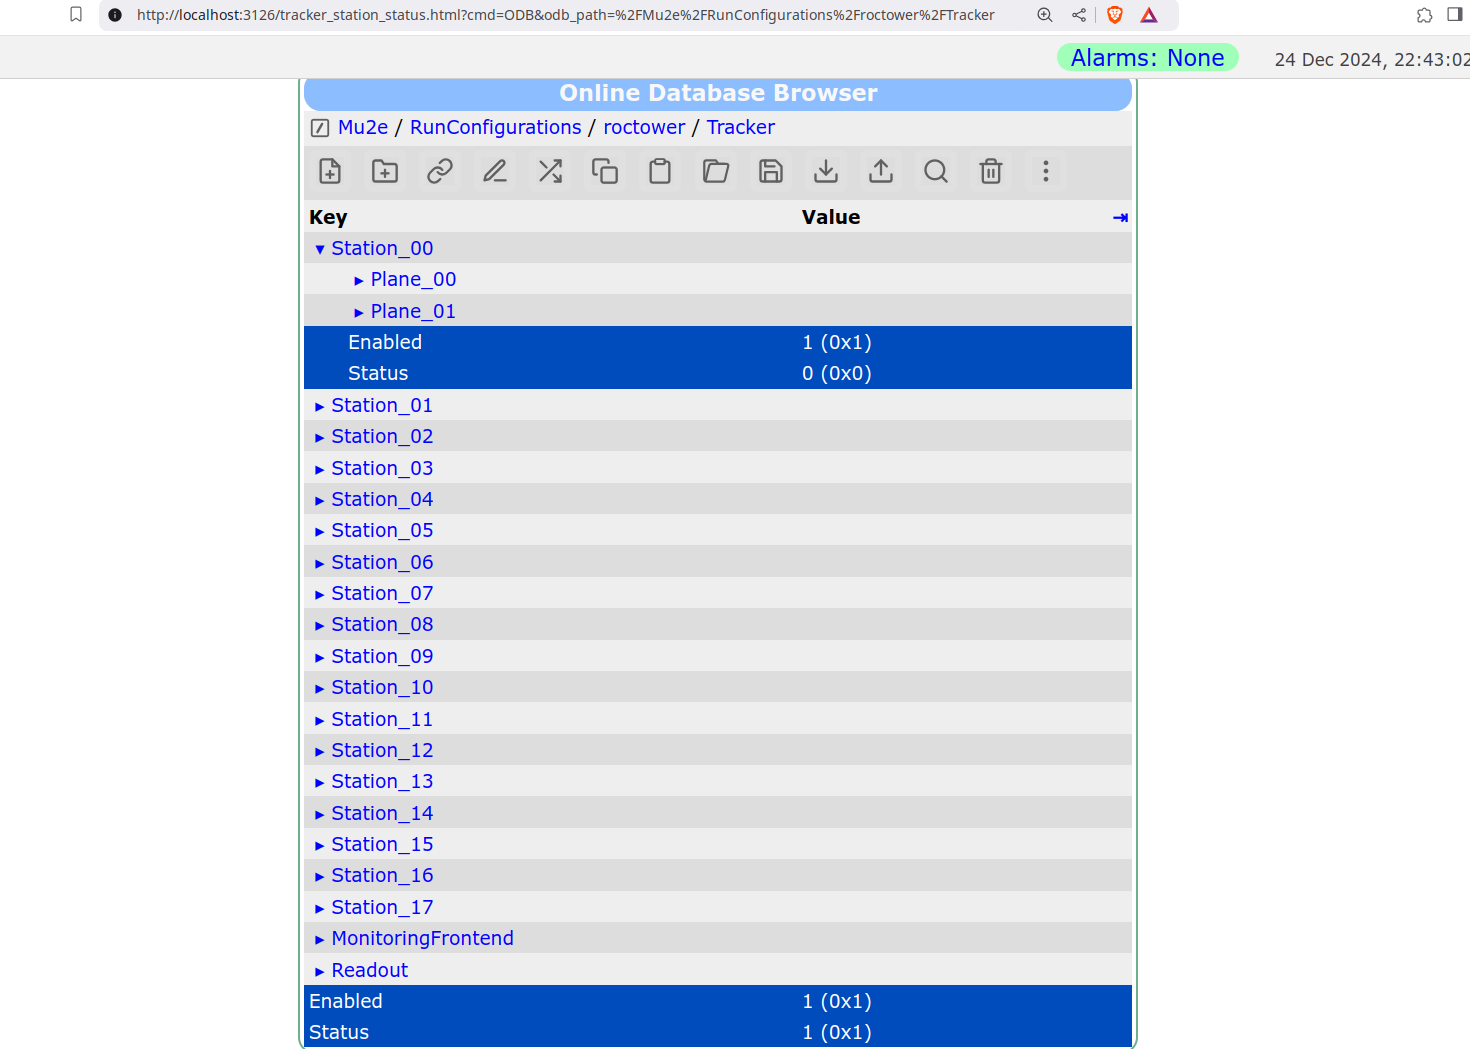
\includegraphics[width=0.95\textwidth]{png/tracker_config}
      }
    };
    % \node [text width=8cm, scale=1.0] at (14.5,0.5) {$\mu_B$, expected background mean};
    % \node [text width=8cm, scale=1.0, rotate={90}] at (1.5,7.5) { $S_{D}$, ``discovery'' signal strength  };
  \end{tikzpicture}
  \caption{
    \label{figure:tracker_config}
    Tracker: configuration levels from the station down to the panel, .
  }
\end{figure}


Lower levels of the tracker configuration hierarchy are shown in Figure~\ref{figure:station_config}.

\begin{figure}[H]
  \begin{tikzpicture}
    \node[anchor=south west,inner sep=0] at (0,0.) {
      % \node[shift={(0 cm,0.cm)},inner sep=0,rotate={90}] at (0,0) {}
      \makebox[\textwidth][c] {
        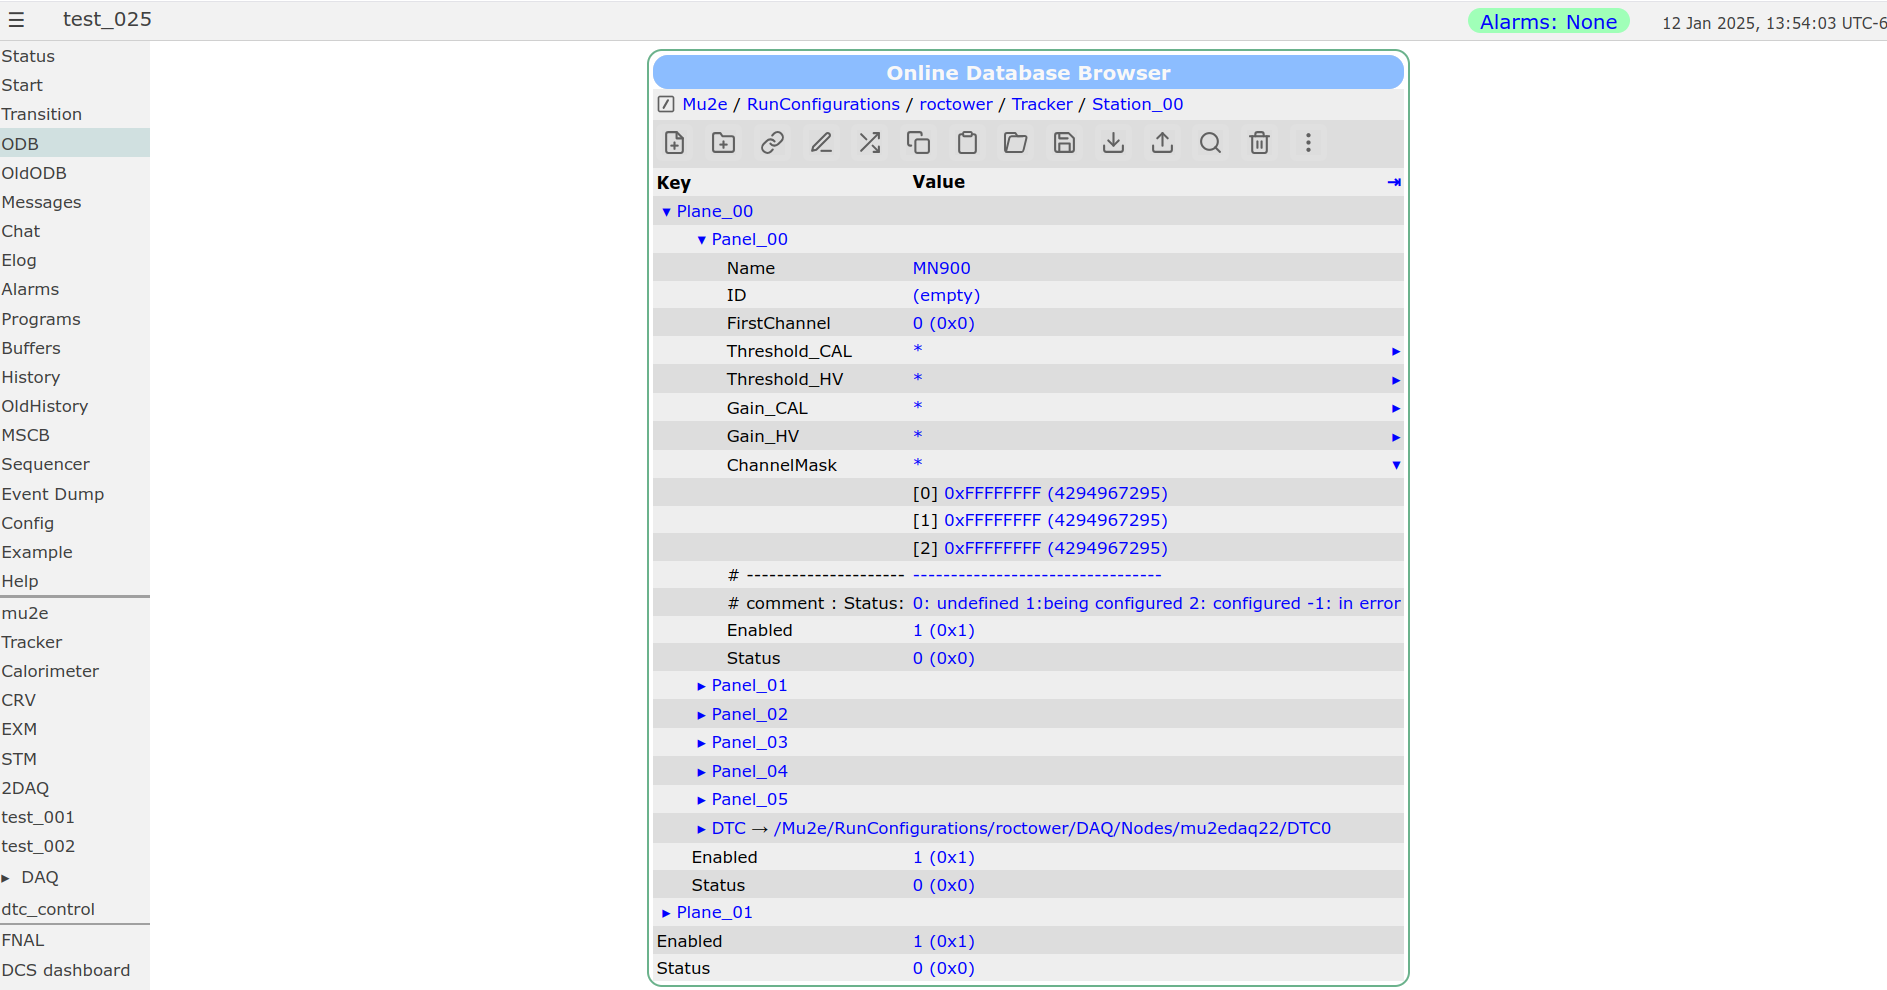
\includegraphics[width=0.95\textwidth]{png/station_config}
      }
    };
    % \node [text width=8cm, scale=1.0] at (14.5,0.5) {$\mu_B$, expected background mean};
    % \node [text width=8cm, scale=1.0, rotate={90}] at (1.5,7.5) { $S_{D}$, ``discovery'' signal strength  };
  \end{tikzpicture}
  \caption{
    \label{figure:station_config}
    Tracker configuration. The tracker, as well as each of the stations, has ``Enabled'' and
    ``Status'' fields.
  }
\end{figure}

%%%%%%%%%%%%%%%%%%%%%%%%%%%%%%%%%%%%%%%%%%%%%%%%%%%%%%%%%%%%%%%%%%%%%%%%%%%%%% 
\subsection{Calorimeter} 


%%%%%%%%%%%%%%%%%%%%%%%%%%%%%%%%%%%%%%%%%%%%%%%%%%%%%%%%%%%%%%%%%%%%%%%%%%%%%% 
\subsection{CRV} 


%%%%%%%%%%%%%%%%%%%%%%%%%%%%%%%%%%%%%%%%%%%%%%%%%%%%%%%%%%%%%%%%%%%%%%%%%%%%%% 
\subsection{STM} 




%%% Local Variables:
%%% mode: latex
%%% TeX-master: t
%%% End:

%%%%%%%%%%%%%%%%%%%%%%%%%%%%%%%%%%%%%%%%%%%%%%%%%%%%%%%%%%%%%%%%%%%%%%%%%%%%%%
\subsection{DAQ}
Top view of the DAQ configuration hierarchy is shown in Figure~\ref{figure:daq_config}.

\begin{figure}[H]
  \begin{tikzpicture}
    \node[anchor=south west,inner sep=0] at (0,0.) {
      % \node[shift={(0 cm,0.cm)},inner sep=0,rotate={90}] at (0,0) {}
      \makebox[\textwidth][c] {
        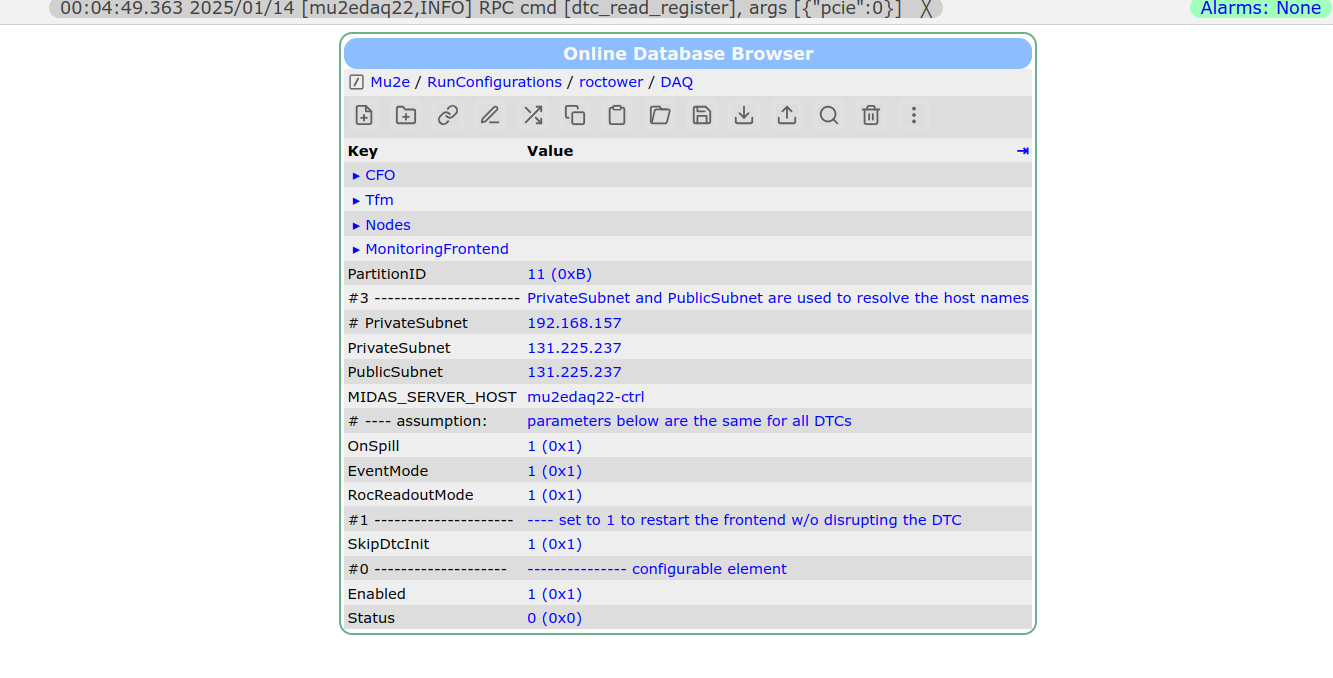
\includegraphics[width=0.95\textwidth]{png/daq_configuration}
      }
    };
    % \node [text width=8cm, scale=1.0] at (14.5,0.5) {$\mu_B$, expected background mean};
    % \node [text width=8cm, scale=1.0, rotate={90}] at (1.5,7.5) { $S_{D}$, ``discovery'' signal strength  };
  \end{tikzpicture}
  \caption{
    \label{figure:daq_config}
    Top level of the DAQ configuration
  }
\end{figure}

It includes configuration of the CFO, the Trigger Farm Manager (TRM), configuration
of the trigger farm nodes and a numebr of global DAQ parameters.


%%%%%%%%%%%%%%%%%%%%%%%%%%%%%%%%%%%%%%%%%%%%%%%%%%%%%%%%%%%%%%%%%%%%%%%%%%%%%%
\newpage
\subsubsection{Emulated CFO configuration}
An example of the emulated CFO configuration is shown in Figure~\ref{figure:cfo_config}.
It includes a link to the configuration of the corresponding FPGA (DTC) 
defined within the same configuration, and a list of the CFO-specific parameters.

\begin{figure}[H]
  \begin{tikzpicture}
    \node[anchor=south west,inner sep=0] at (0,0.) {
      % \node[shift={(0 cm,0.cm)},inner sep=0,rotate={90}] at (0,0) {}
      \makebox[\textwidth][c] {
        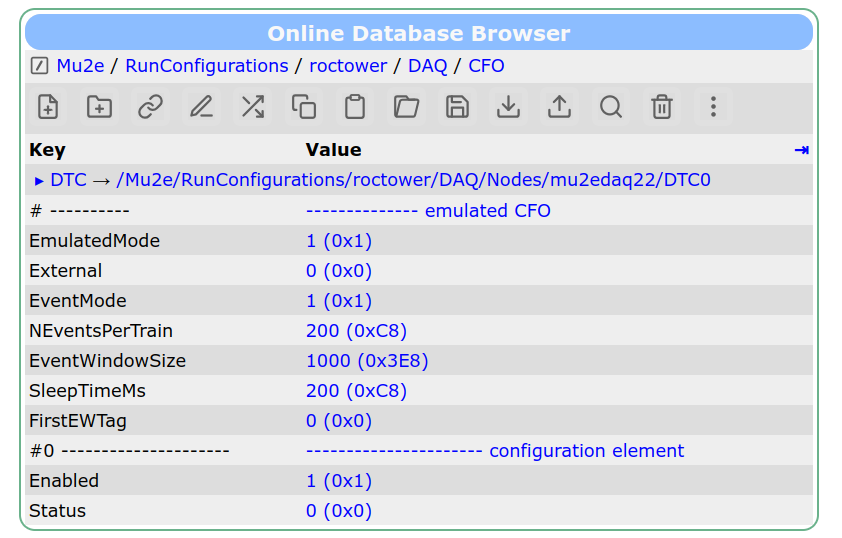
\includegraphics[width=0.95\textwidth]{png/cfo_configuration}
      }
    };
    % \node [text width=8cm, scale=1.0] at (14.5,0.5) {$\mu_B$, expected background mean};
    % \node [text width=8cm, scale=1.0, rotate={90}] at (1.5,7.5) { $S_{D}$, ``discovery'' signal strength  };
  \end{tikzpicture}
  \caption{
    \label{figure:cfo_config}
    CFO configuration
  }
\end{figure}

%%%%%%%%%%%%%%%%%%%%%%%%%%%%%%%%%%%%%%%%%%%%%%%%%%%%%%%%%%%%%%%%%%%%%%%%%%%%%%
\newpage
\subsubsection{Hardware CFO configuration}

\add{To be added}

% \begin{figure}[H]
%   \begin{tikzpicture}
%     \node[anchor=south west,inner sep=0] at (0,0.) {
%       % \node[shift={(0 cm,0.cm)},inner sep=0,rotate={90}] at (0,0) {}
%       \makebox[\textwidth][c] {
%         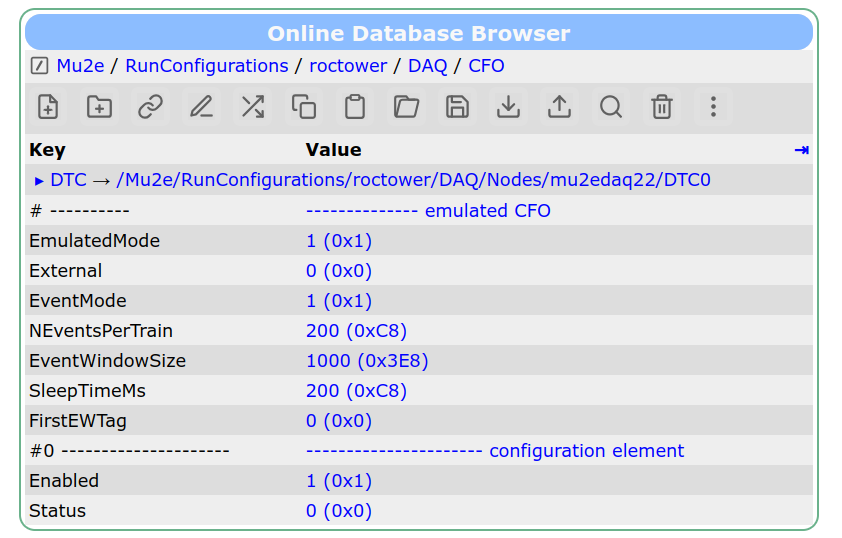
\includegraphics[width=0.95\textwidth]{png/cfo_configuration}
%       }
%     };
%     % \node [text width=8cm, scale=1.0] at (14.5,0.5) {$\mu_B$, expected background mean};
%     % \node [text width=8cm, scale=1.0, rotate={90}] at (1.5,7.5) { $S_{D}$, ``discovery'' signal strength  };
%   \end{tikzpicture}
%   \caption{
%     \label{figure:cfo_config}
%     CFO configuration
%   }
% \end{figure}
% 

%%%%%%%%%%%%%%%%%%%%%%%%%%%%%%%%%%%%%%%%%%%%%%%%%%%%%%%%%%%%%%%%%%%%%%%%%%%%%%
\subsubsection{DAQ-specific frontends}

\begin{itemize}
\item
  one monitoring/control frontend per DAQ server. Monitoring:
  \begin{itemize}
  \item
    2 DTC's with 6 ROCs per DTC
  \item
    ARTDAQ processes:
    \begin{itemize}
    \item
      2 boardreaders, N event builders, potentially a data logger, and a dispatcher
    \end{itemize}
  \item
    overall health: amount of free space available
  \end{itemize}
\item
  emulated CFO:
  \begin{itemize}
  \item
    currently : a separate frontend 
  \item 
    make the CFO frontend a separate thread of the node frontend
  \end{itemize}
\item
  external CFO frontend 
\item
  global control frontend:
\end{itemize}

%%%%%%%%%%%%%%%%%%%%%%%%%%%%%%%%%%%%%%%%%%%%%%%%%%%%%%%%%%%%%%%%%%%%%%%%%%%%%%
\subsection{ARTDAQ configuration}

ARTDAQ configuration is stored in ODB. It consists of two parts:
\begin{itemize}
\item
  Trigger Farm Manager (TFM) configuration
\item
  configuration of the artdaq processes on each farm node
\end{itemize}

A configuration of a single node is shown in Figure ~\ref{figure:artdaq_configuration}.

\begin{figure}[H]
  \begin{tikzpicture}
    \node[anchor=south west,inner sep=0] at (0,0.) {
      % \node[shift={(0 cm,0.cm)},inner sep=0,rotate={90}] at (0,0) {}
      \makebox[\textwidth][c] {
        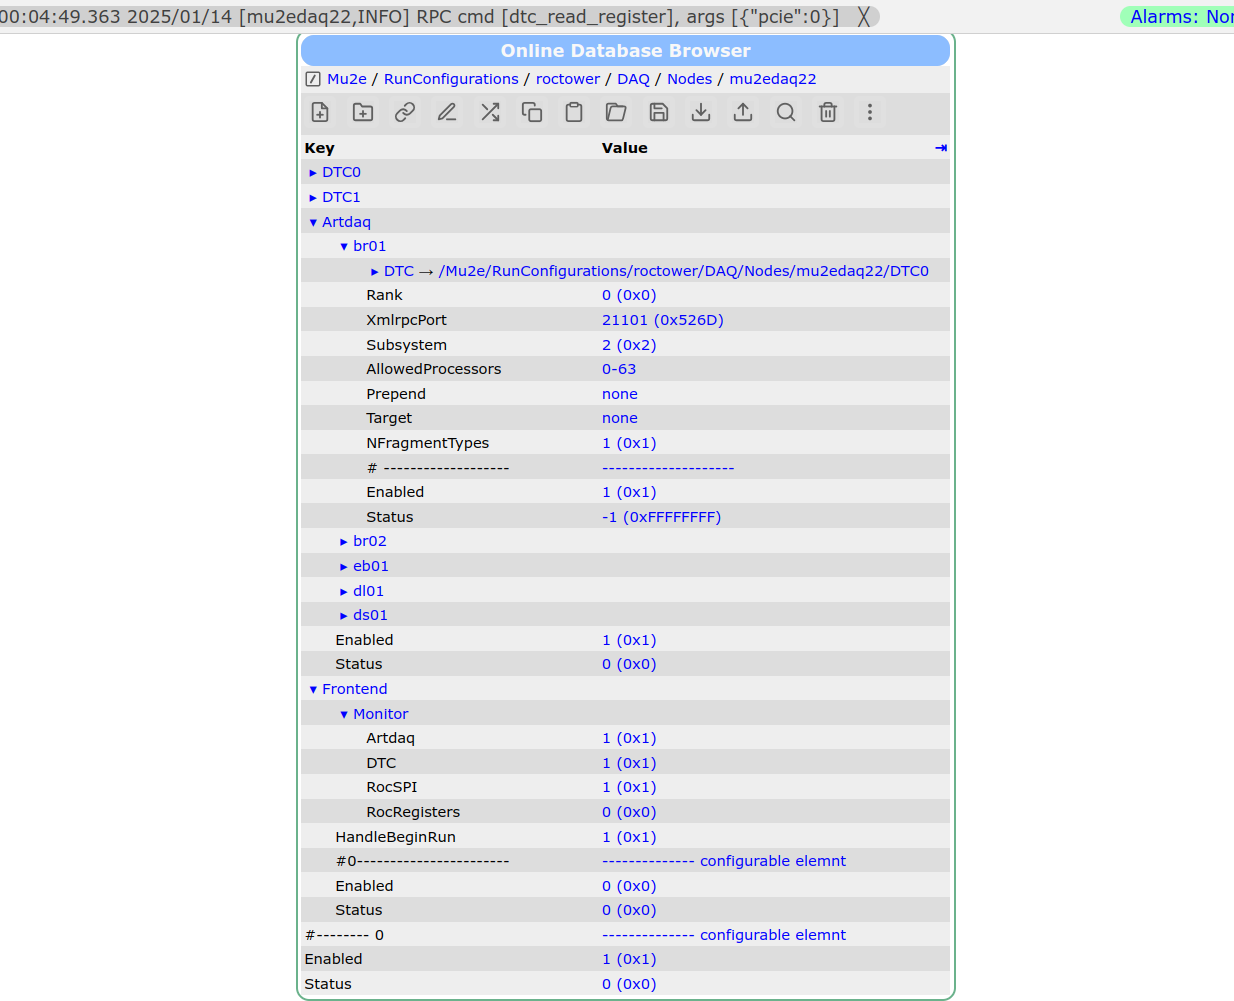
\includegraphics[width=0.95\textwidth]{png/artdaq_configuration}
      }
    };
    % \node [text width=8cm, scale=1.0] at (14.5,0.5) {$\mu_B$, expected background mean};
    % \node [text width=8cm, scale=1.0, rotate={90}] at (1.5,7.5) { $S_{D}$, ``discovery'' signal strength  };
  \end{tikzpicture}
  \caption{
    \label{figure:artdaq_configuration}
    CFO configuration
  }
\end{figure}

It has
\begin{itemize}
\item
  parameters of the DTCs. There could be zero, one, or two DTCs on a farm node.
\item
  parameters of the artdaq processes running on that node.
  Configuration of the ARTDAQ boardreaders has links to the definitions
  of the DTCs they are reading. A boardreader need to know the PCIE address of the DTC
  it is interacting with. At start time, the boardreaders query that information
  from the ODB.
  
\item
  parameters of the node control frontend, including the configuration of the
  slow controls ("Frontend/Monitor")
\end{itemize}

%%%%%%%%%%%%%%%%%%%%%%%%%%%%%%%%%%%%%%%%%%%%%%%%%%%%%%%%%%%%%%%%%%%%%%%%%%%%%%
\subsection{DAQ-to-subdetectors interface}
The DAQ elements are "mapped" linked to the corresponding subdetector elements using ODB links,
as shown in Figure ~\ref{figure:daq_to_tracker_interface}.
\begin{figure}[H]
  \begin{tikzpicture}
    \node[anchor=south west,inner sep=0] at (0,0.) {
      % \node[shift={(0 cm,0.cm)},inner sep=0,rotate={90}] at (0,0) {}
      \makebox[\textwidth][c] {
        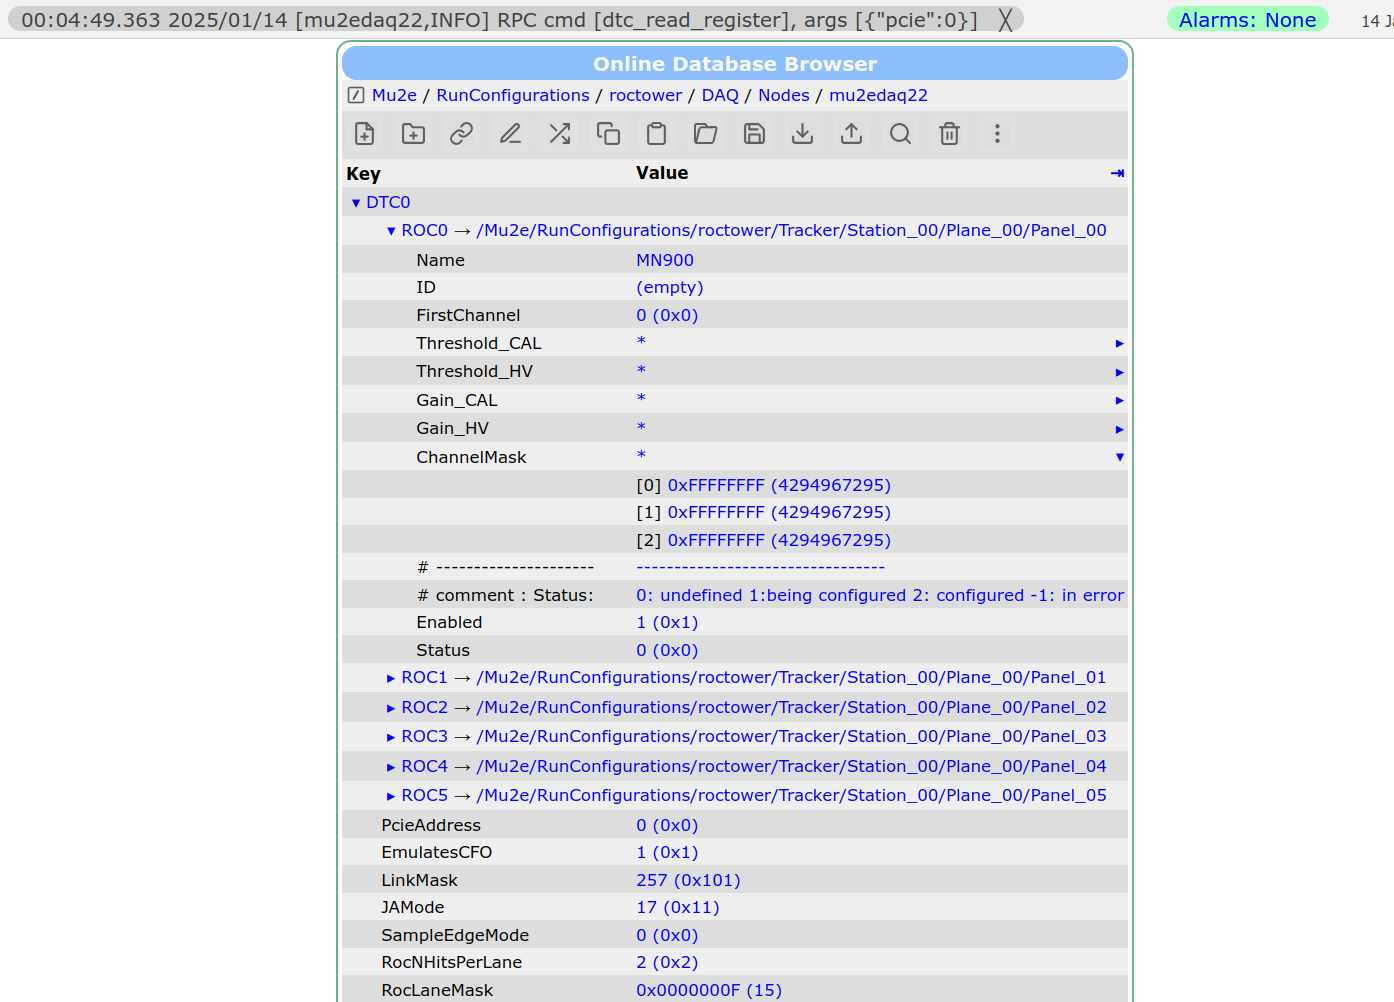
\includegraphics[width=0.95\textwidth]{png/daq_to_tracker_interface}
      }
    };
    % \node [text width=8cm, scale=1.0] at (14.5,0.5) {$\mu_B$, expected background mean};
    % \node [text width=8cm, scale=1.0, rotate={90}] at (1.5,7.5) { $S_{D}$, ``discovery'' signal strength  };
  \end{tikzpicture}
  \caption{
    \label{figure:daq_to_tracker_interface}
    CFO configuration
  }
\end{figure}

A DAQ node has links to the DTCs installed on that node, and the tracker DTC ROCs shown have
links to the definitions of the tracker panels they are reading.

%%% Local Variables:
%%% mode: latex
%%% TeX-master: t
%%% End:

% \section{Interface to ARTDAQ}

ARTDAQ processes are controlled by the special MIDAS ``
Trigger Farm Manager (TFM) frontend'', tfm\_launch\_fe.py.

The TFM frontend runs the TFM manager which inherits the functionality
of artdaq\_daqinterface, providing an interface between the MIDAS-based
run control system and ARTDAQ.

The TFM reads its initial settings from ODB. its configuration path is "/Mu2e/ActiveRunConfiguration/DAQ/Tfm"


%%% Local Variables:
%%% mode: latex
%%% TeX-master: t
%%% End:



%%%%%%%%%%%%%%%%%%%%%%%%%%%%%%%%%%%%%%%%%%%%%%%%%%%%%%%%%%%%%%%%%%%%%%%%%%%%%%
\section{Monitoring of the detector}

At run-time, the status of the detecotr is visualized by the system status tree.
The top page of the tree is shown in Figure~\ref{figure:mu2e_status_page}.

\begin{itemize}
\item
  one monitoring frontend per DAQ node, monitors the DTCs and the ARTDAQ processes.
  The frontend is responsible for setting status of the ROCs, boardreaders, and such.
  THe same frontend propagates the error status up the subdetector tree. 
  \item
  monitoring GUI - displays status of the detector. MIDAS-based javascript+HTML.
  Each element of the detector system, as described in ODB, in addition to other parameters
  has two mandatory ones: ``Enabled'' and ``Status''.
  \begin{itemize}
  \item 
    Setting Enabled=0 excludes the element from the configuration, in which case it will be
    shown in gray.
  \item
    Enabled=1 will result in the element shown in green (Status >= 0) or red (Status< 0) 
  \end{itemize}
\end{itemize}

\begin{figure}[H]
  \begin{tikzpicture}
    \node[anchor=south west,inner sep=0] at (0,0.) {
      % \node[shift={(0 cm,0.cm)},inner sep=0,rotate={90}] at (0,0) {}
      \makebox[\textwidth][c] {
        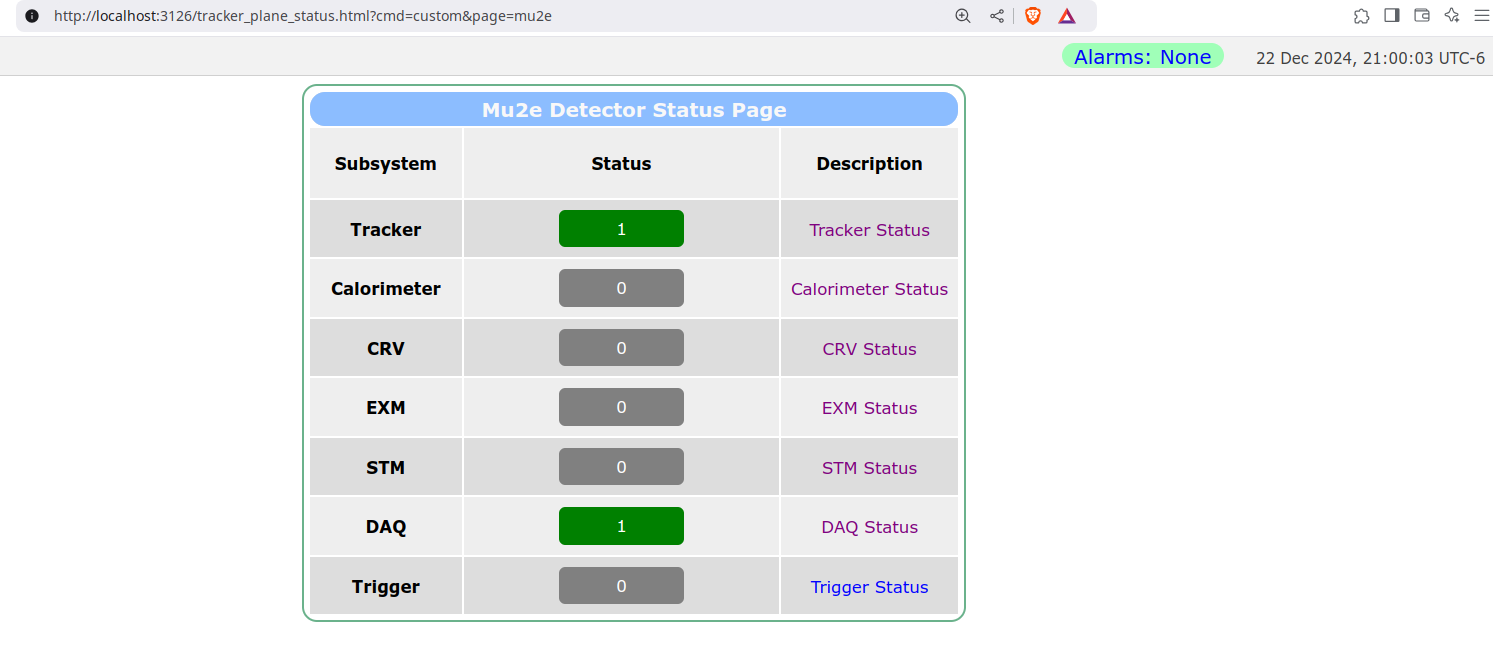
\includegraphics[width=0.95\textwidth]{png/mu2e_status_page}
      }
    };
    % \node [text width=8cm, scale=1.0] at (14.5,0.5) {$\mu_B$, expected background mean};
    % \node [text width=8cm, scale=1.0, rotate={90}] at (1.5,7.5) { $S_{D}$, ``discovery'' signal strength  };
  \end{tikzpicture}
  \caption{
    \label{figure:mu2e_status_page}
    Mu2e status page (prototype)
  }
\end{figure}

State of each enabled configurable element is monitored by a MIDAS frontend.
If a problem is detected, the status of the element is set to a negative
number, which value represents the status code of the problem.

A special configuration frontend propagates the status of the problem up the
configuration tree in ODB. For example, if a problem is detected with one of the
tracker panels, the status box corresponding to the tracker on the top monitoring
page will also become red.

Figure~\ref{figure:daq_status} shows the prototype of the DAQ monitoring page.
The screenshot has been takes after the end of one of the test runs.
One of the mu2edaq22 boardreaders is ``in the red'' because one the ROCs it
was reading timed out.

\begin{figure}[H]
  \begin{tikzpicture}
    \node[anchor=south west,inner sep=0] at (0,0.) {
      % \node[shift={(0 cm,0.cm)},inner sep=0,rotate={90}] at (0,0) {}
      \makebox[\textwidth][c] {
        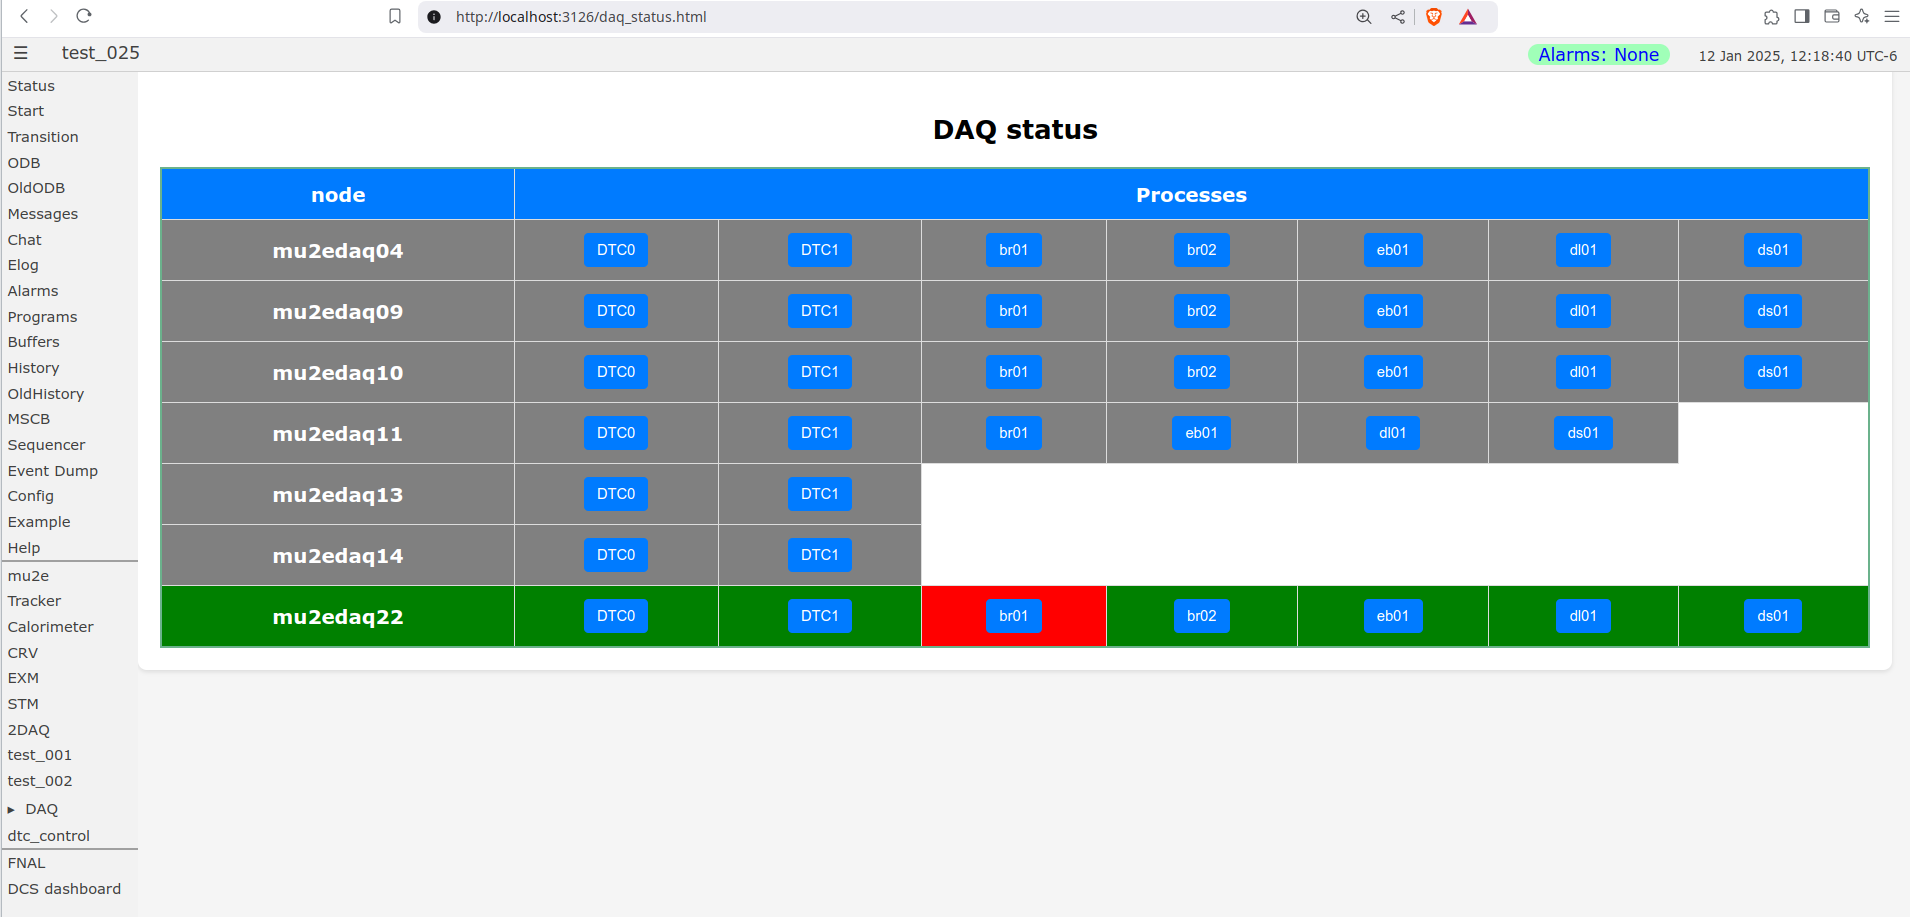
\includegraphics[width=0.95\textwidth]{png/daq_status}
      }
    };
    % \node [text width=8cm, scale=1.0] at (14.5,0.5) {$\mu_B$, expected background mean};
    % \node [text width=8cm, scale=1.0, rotate={90}] at (1.5,7.5) { $S_{D}$, ``discovery'' signal strength  };
  \end{tikzpicture}
  \caption{
    \label{figure:daq_status}
    Prototype of the DAQ status page
  }
\end{figure}

After a problem with the ROC is cleared, and the readout resumes, the boardreader status
is set to zero by the monitoring frontend, and the color of the corresponding box changes to green.
The change is propagated up the configuration tree by the configuration frontend,
and the color of the DAQ monitoring box becomes green again.

%%%%%%%%%%%%%%%%%%%%%%%%%%%%%%%%%%%%%%%%%%%%%%%%%%%%%%%%%%%%%%%%%%%%%%%%%%%%%%
\section{Interaction with the hardware}

Interaction with the hardware is handled by the node frontends.

If manual interaction is required, a click on the DTC button on the DAQ monitoring
page shown in Figure~\ref{figure:daq_status} opens a DTC control page, prototype of which
is shown in  Figure~\ref{figure:dtc_control_page}. Parameters of the commands to be executed
are stored of ODB in the "/Mu2e/Commands" subtree and could be set interactively
via either a web-based interface or {\bf odbedit}. 

\begin{figure}[H]
  \begin{tikzpicture}
    \node[anchor=south west,inner sep=0] at (0,0.) {
      % \node[shift={(0 cm,0.cm)},inner sep=0,rotate={90}] at (0,0) {}
      \makebox[\textwidth][c] {
        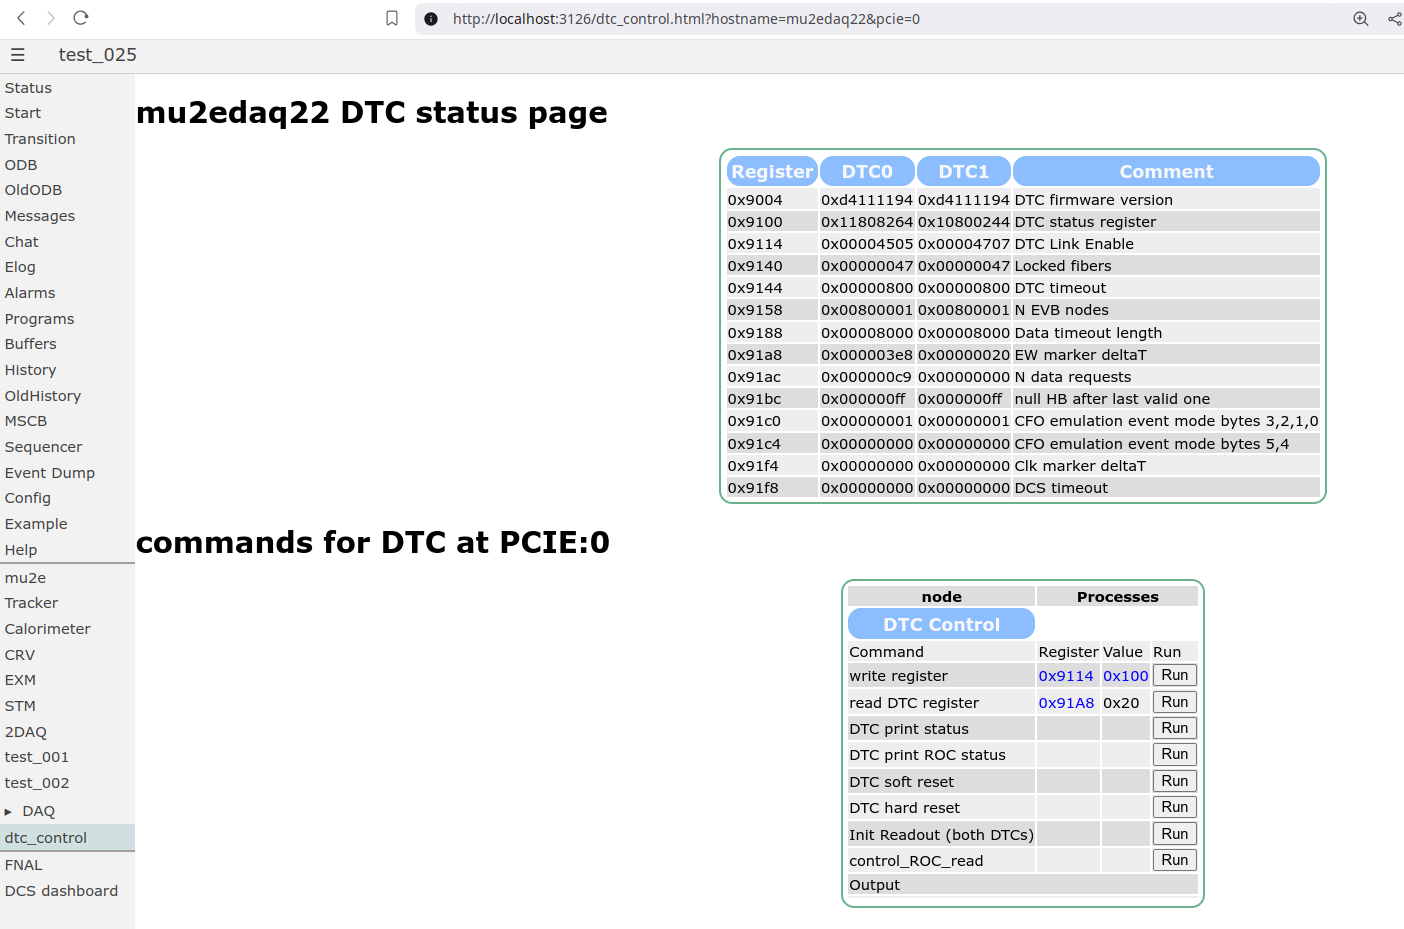
\includegraphics[width=0.95\textwidth]{png/dtc_control_page}
      }
    };
    % \node [text width=8cm, scale=1.0] at (14.5,0.5) {$\mu_B$, expected background mean};
    % \node [text width=8cm, scale=1.0, rotate={90}] at (1.5,7.5) { $S_{D}$, ``discovery'' signal strength  };
  \end{tikzpicture}
  \caption{
    \label{figure:dtc_control_page}
    Prototype of the DTC control page
  }
\end{figure}
%%% Local Variables:
%%% mode: latex
%%% TeX-master: t
%%% End:

%%%%%%%%%%%%%%%%%%%%%%%%%%%%%%%%%%%%%%%%%%%%%%%%%%%%%%%%%%%%%%%%%%%%%%%%%%%%%%
\section{Operational procedures and details}

\section{Starting and stopping a run }

\begin{itemize}
\item
  request the next run number from the Mu2e run conditions database
  (MIDAS sequencer ==> config/scripts/get\_next\_run\_number.py) and store
  it in ODB (rn-1)
\item
  configure the detector using the sequencer scripts.
  When the system will become stable enough, the configuration functionality
  could be gradually moved to frontends.
\item
  start the run. At this point the detector is configured and ready to be read out.
  The TFM frontend starts the ARTDAQ processes , after which the CFO frontend 
  initiates new run plan.
\item
  to stop the run, the CFO frontend terminates execution of the run plan
  by the CFO, after that the TFM frontend ends the run and the TFM terminates
  the ARTDAQ processes.
\end{itemize}

%%%%%%%%%%%%%%%%%%%%%%%%%%%%%%%%%%%%%%%%%%%%%%%%%%%%%%%%%%%%%%%%%%%%%%%%%%%%%%
\subsection{Host Names}

A DAQ host is typically simultaneously connected to several subnets and on
those subnets it may have different names.
For example, TCP traffic on a public network may be partially blocked,
in which case the DAQ communication has to be using a private network.

\begin{itemize}
\item
  "/Mu2e/ActiveRunConfiguration/DAQ/PublicSubnet"  :
  defines the host name used for labeling the host in ODB
\item
  "/Mu2e/ActiveRunConfiguration/DAQ/PrivateSubnet" :
  defines the host name used for defining the IPs
\end{itemize}

Usually the ``public'' names are shorter.


%%%%%%%%%%%%%%%%%%%%%%%%%%%%%%%%%%%%%%%%%%%%%%%%%%%%%%%%%%%%%%%%%%%%%%%%%%%%%%
\subsubsection{Naming conventions for ARTDAQ components}

It is assumed that :
\begin{itemize}
\item 
  artdaq boardreaders described in the configuration have names "br01", "br02", etc
\item 
  artdaq event builders have names "eb01", "eb02", etc
\item 
  artdaq data loggers have names "dl01", "dl02", etc
\item 
  artdaq dispatchers have names "ds01", "ds02", etc
\end{itemize}

This convention allows to use the ARTDAQ component names, as is, in the monitoring system.

%%%%%%%%%%%%%%%%%%%%%%%%%%%%%%%%%%%%%%%%%%%%%%%%%%%%%%%%%%%%%%%%%%%%%%%%%%%%%%
\subsection{Port assignment for ARTDAQ XMLRPC communication}

ARTDAQ convention: for a given partition, the first port number is base\_port=10000+1000*PARTITION
\begin{itemize}
\item
  boardreaders: base\_port+101 - base\_port+199\\
  expect the total number of boardreaders in the system to be < 100 \\
  The XMLRPC port of 'br01' is base\_port+101
\item
  filters (event builders) : base\_port+201 - base\_port+299
  The XMLRPC port of 'eb01' is base\_port+201
\item
  data loggers: base\_port+301 - base\_port+399
  The XMLRPC port of 'dl01' is base\_port+301
\item
  dispatchers: base\_port+401 - base\_port+499
  The XMLRPC port of 'ds01' is base\_port+301
\end{itemize}

%%% Local Variables:
%%% mode: latex
%%% TeX-master: t
%%% End:

%%%%%%%%%%%%%%%%%%%%%%%%%%%%%%%%%%%%%%%%%%%%%%%%%%%%%%%%%%%%%%%%%%%%%%%%%%%%%%
\section{Documentation and support considerations}

\begin{itemize}
\item
  MIDAS wiki \cite{2025_MIDAS_WIKI}, hosted by TRIUMF, serves the role of 
  of the user/developer manuals which is always up to date.
\item 
  The MIDAS forum provides an efficient way for communicating with the experts.
\item
  MIDAS is supported on Windows, Macs and Linux.
  Expect active support to continue over the lifetime of Mu2e.
\item 
  MIDAS codebase is public and maintained at: https://bitbucket.org/tmidas/workspace/projects/PROJ
\item
  significant developer base: about 4-5 core developers from several running experiments
\item
  activity over the last 12 months: 100's of commits by the core developers/maintainers plus
  13 pull requests by 6 developers
\end{itemize}




%%% Local Variables:
%%% mode: latex
%%% TeX-master: t
%%% End:

%%%%%%%%%%%%%%%%%%%%%%%%%%%%%%%%%%%%%%%%%%%%%%%%%%%%%%%%%%%%%%%%%%%%%%%%%%%%%% 
\section {Summary}

\begin{itemize}
\item 
  The MIDAS+ARTDAQ solution for the Mu2e DAQ has been extensively prototyped
  over the last several months.
\item
  the functionality of the described system, in many aspects,
  already exceeds that of the OTSDAQ-based system  
\item
  the system is significantly simpler than the OTSDAQ-based solution,
  for both users and developers
\item
  collaboration members, including students, are contributing
  to the development process. 
\item
  new collaboration members joining Mu2e from other muon experiments
  will more likely be familiar with a MIDAS-based DAQ than with
  any other DAQ system
\end{itemize}

Based on our assessment, a combination of MIDAS and ARTDAQ provides
the solution for the Mu2e DAQ which the collaboration will be able
to maintain and operate over the course of the Mu2e data taking.

\vspace{0.2in}
We therefore propose to exercise the MIDAS+ARTDAQ based DAQ system
in the upcoming GR4 to further test its functionality and determine
next steps. 

%%% Local Variables:
%%% mode: latex
%%% TeX-master: t
%%% End:

%%%%%%%%%%%%%%%%%%%%%%%%%%%%%%%%%%%%%%%%%%%%%%%%%%%%%%%%%%%%%%%%%%%%%%%%%%%%%%
\section{APPENDIX: comparison to OTSDAQ}

\tiny{
  \begin{verbatim}
|---------------+----------------------------------------------+-----------------------------------------|
| aadf          | --------------OTS --------------             | --------------- MIDAS ----------------- |
|---------------+----------------------------------------------+-----------------------------------------|
| data model    | none, no concept of the user monitoring      | ODB stores everything                   |
|               | data being stored / updated at run-time      |                                         |
|               | SQL tables stored in json structures         | a json structure                        |
|---------------+----------------------------------------------+-----------------------------------------|
| documentation | none                                         | MIDAS website + examples                |
|---------------+----------------------------------------------+-----------------------------------------|
|               | DTCFrontEndInterface                         |                                         |
| inheritance   | -> CFOandDTCCoreVInterface -> FEVInterface   |                                         |
| from the      | -> ( WorkLoop, Configurable, VStateMachine)  |                                         |
| whole world   | Workloop ->  virtual toolbox::lang::Class    |                                         |
|               |                                              |                                         |
|               | everything depends on everything else        |                                         |
|---------------+----------------------------------------------+-----------------------------------------|
| configuration | impenetrable                                 | clean                                   |
|---------------+----------------------------------------------+-----------------------------------------|
| client-server | OTS doesn't have clients , user applications | clients connect to server, independent  |
|               | are loaded dynamically                       | on                                      |
|               | crash of a user app crashes the server       |                                         |
|---------------+----------------------------------------------+-----------------------------------------|
| ARTDAQ        | ARTDAQ processes don't talk back to OTS      | ARTDAQ run-time info is stored in ODB   |
|---------------+----------------------------------------------+-----------------------------------------|
| FCL files     | no way to change a parameter manually        | runs from static FCL files              |
|---------------+----------------------------------------------+-----------------------------------------|
| symlinks      | lots                                         | none                                    |
|---------------+----------------------------------------------+-----------------------------------------|
| expertise     | 1 person                                     | many developers, many users             |
|               |                                              |                                         |
  \end{verbatim}
}



\begin{itemize}
\item
  aaaa
\end{itemize}
%%% Local Variables:
%%% mode: latex
%%% TeX-master: t
%%% End:

%%%%%%%%%%%%%%%%%%%%%%%%%%%%%%%%%%%%%%%%%%%%%%%%%%%%%%%%%%%%%%%%%%%%%%%%%%%%%% 
%
%%%%%%%%%%%%%%%%%%%%%%%%%%%%%%%%%%%%%%%%%%%%%%%%%%%%%%%%%%%%%%%%%%%%%%%%%%%%%%
\newpage
\bibliographystyle{unsrtnat}
\bibliography{clfv,mu2e_internal_notes,daq}

% \include{appendix_a}
\include{appendix_b}

\end{document}
